\documentclass[
11pt,
fleqn,
titlepage]{article}

% Packages

\usepackage{authblk}
\usepackage[sfdefault]{roboto}
\usepackage{pgfplots}
\pgfplotsset{
    compat=1.18,
    title style={font=\footnotesize},
    tick label style={font=\small},
    label style={font=\small},
    legend style={font=\footnotesize}}
\usetikzlibrary{intersections}
\usepackage[a4paper, headheight=14pt]{geometry}
\usepackage[document]{ragged2e}
\usepackage{parskip}
\usepackage[babel, tracking, verbose]{microtype}
\usepackage[defaultlines=2, all]{nowidow}
\usepackage{enumitem}
\usepackage{subcaption}
\captionsetup{
    labelfont=bf,
    singlelinecheck=false,
    justification=RaggedRight}
\captionsetup[subfigure]{
    labelformat=brace}
\renewcommand\thesubfigure{\roman{subfigure}}
\usepackage{polyglossia}
\setdefaultlanguage[variant=american]{english}
\usepackage{csquotes}
\usepackage[style=apa]{biblatex}
\addbibresource{bibliography.bib}
\usepackage{fancyhdr}
\usepackage{pdfpages}
\usepackage{mathtools}
\usepackage{amsthm}
\usepackage[
math-style=ISO,
warnings-off={mathtools-colon, mathtools-overbracket}
]{unicode-math}
\usepackage{nicefrac}
\usepackage[renew-dots, renew-matrix]{nicematrix}
\NiceMatrixOptions{cell-space-limits = 1pt}
\usepackage{booktabs}
\usepackage[labelfont=bf]{caption}
\usepackage{threeparttablex}
\usepackage{siunitx}
\usepackage[imakeidx]{xindex}
\makeindex[intoc]
\usepackage[pdfa]{hyperref}
\usepackage{colorprofiles}
\hypersetup{
    pdfinfo={
        Title={Analysis of differential gene expression in wild and cultivated rice under drought stress},
        Author={Ingo Giebel},
        Subject={Student work QBio304: Applied Bioinformatics},
        Keywords={Heinrich-Heine-Universität Düsseldorf, WS 2022/2023, QBio304: Applied Bioinformatics, Student work, Instructors: Prof. Dr. Björn Usadel, Dr. Jedrzej Jakub Szymanski}},
        colorlinks,
        linkcolor=blue,
        linktoc=all}
\usepackage[ocgcolorlinks, tikz]{ocgx2}
\sloppy

% Header

\pagestyle{fancy}
\fancyhf{}
\fancyhead[L]{Student work QBio304: Applied Bioinformatics}
\fancyhead[R]{\thepage}
\fancypagestyle{plain}{}

% Title & author

\title{Analysis of differential gene expression in wild and cultivated rice under drought stress}
\author[1]{Ingo Giebel}
\affil[1]{Math.-Nat. Fakultät, Heinrich-Heine-Universität Düsseldorf}
\affil[1]{QBio304: Applied Bioinformatics}
\affil[2]{RG Network Analysis and Modelling, Leibniz Institute of Plant Genetics and Crop Plant Research}
\affil[2]{IBG-4: Bioinformatik, Forschungszentrum Jülich GmbH}
\affil[1]{Prof. Dr. Björn Usadel}
\affil[2]{Dr. Jedrzej Jakub Szymanski}
\date{May 1, 2023}

\begin{document}
    \maketitle

    \tableofcontents

    \newpage
    \listoffigures
    \listoftables

    \newpage
    \section{Abstract}

TODO: Provide a brief summary of the purpose of the assignment, the methods used, the main findings, and the significance of the results. Limit the abstract to 200-250 words.

    \section{Introduction}

RNA-sequencing is used to analyze the transcriptome\index{transcriptome}, indicating which of the genes encoded in the DNA are turned on or off and to what extent. This study examines the impact of drought stress on the gene expression of wild and and cultivated rice, using statistical methods. To this end, publicly available RNA-seq\index{RNA-seq} data from the Institute of Botany, Chinese Academy of Sciences, submitted on January 1st, 2021, is analyzed with respect to differential gene expression. This data allows for a direct comparison of normal and drought stress conditions for the two closely related species of wild and cultivated rice.

    \section{Materials and methods}

\subsection{Selection of the RNA-seq data}

This study uses publicly available paired-end RNA-seq\index{RNA-seq} data of wild and cultivated rice, submitted in January 1, 2021 by the Institute of Botany, Chinese Academy of Sciences. This data allows to compare rice grown under normal conditions with rice grown under drought stress conditions. Furthermore, the data allows for an interspecies comparison of wild rice (Oryza nivara\index{Oryza!nivara}, cultivars BJ278\index{cultivar!BJ278} and BJ89\index{cultivar!BJ89}) with cultivated rice (Oryza sativa\index{Oryza!sativa}, cultivar Nipponbare\index{cultivar!Nipponbare}).

All samples were uniformly taken from seedlings (leaf tissue) at the age of twelve days. Used sequencing platform: Illumina HiSeq 2000\index{Illumina!HiSeq 2000}.

Therefore, the data is well-suited for a targeted analysis of drought stress responses.


\subsection{Quality evaluation}

The quality of the raw and trimmed RNA-seq data\index{RNA-seq!quality assessment} was assessed using FastQC\index{FastQC} \autocite{babraham}. FastQC is a quality control analysis tool for high throughput sequencing data. It provides information about
\begin{itemize}
    \item basic statistics: some simple composition statistics for the FASTQ\index{FASTQ} file analyzed
    \item per base sequence quality: an overview of the range of quality values across all bases at each position in the FASTQ file
    \item per tile sequence quality: an overview of the per tile sequence quality in case an Illumina library was used
    \item per sequence quality scores: an overview of how the overall quality scores of the sequences are distributed
    \item per base sequence content: an overview of the proportion of each base position in a FASTQ file for which each of the four normal DNA bases has been called
    \item per sequence GC content: the GC content across the whole length of each sequence in a file compared with a normal distributed GC content
    \item per base N content: an overview of the N content at each position across all bases
    \item sequence length distribution: an overview of how the sequence lengths are distributed
    \item sequence duplication levels: an overview of the degree of duplication for every sequence in a library
    \item over-represented sequences: a list of over-represented sequences matched against common contaminants\index{RNA-seq!contaminant}
    \item adapter content: a check for significant amounts of adapter sequences\index{RNA-seq!adapter sequence} the FASTQ file
\end{itemize}

The results of the separate FastQC analyses (of the raw and trimmed FASTQ files), the results of the Trimmomatic\index{Trimmomatic} trimming and the information about the kallisto\index{kallisto} pseudoalignments\index{transcript!pseudoalignment} were summarized in an interactive MultiQC\index{MultiQC} HTML-report. See \autocite{10.1093/bioinformatics/btw354}.


\subsection{RNA-seq preprocessing}

The initial quality assessment of the raw FASTQ files revealed that about roughly the first 12 base pairs of the reads were of low quality. Therefore, the data was preprocessed/trimmed using Trimmomatic\index{Trimmomatic}, a "flexible and efficient preprocessing tool, which could correctly handle paired-end data" \autocite{10.1093/bioinformatics/btw354}.

That trimming substantially improved the per base sequence content and the per base sequence quality. Figures \ref{fig:0.1-FastQC-per_base_seq_cont-CRR240976-raw_vs_trim} and \ref{fig:0.1-FastQC-per_base_seq_qual-CRR240976-raw_vs_trim} show exemplary a comparison of the FastQC assessments of a raw FASTQ file vs the corresponding trimmed FASTQ file.

\begin{figure}[htbp]
    \caption{FastQC quality assessment of the per base sequence content of the raw FASTQ file CRR240976\_f1.fastq.gz vs the trimmed file CRR240976\_f1.trim.p.fastq.gz}
    \label{fig:0.1-FastQC-per_base_seq_cont-CRR240976-raw_vs_trim}
    \begin{subfigure}[t]{0.48\linewidth}
        \caption{Raw data}
        \label{fig:0.1-FastQC-per_base_seq_cont-CRR240976}
        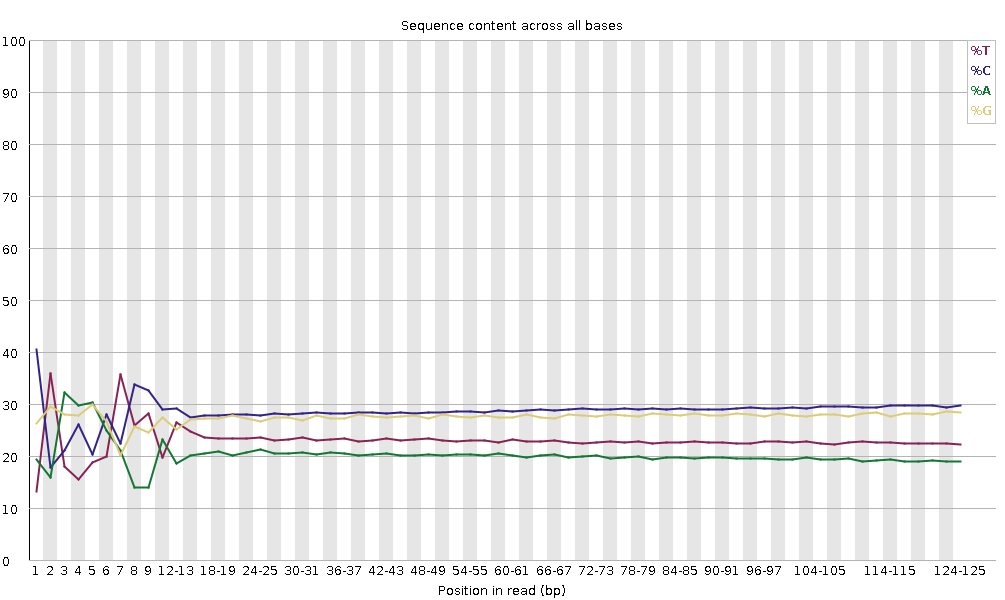
\includegraphics[width=\textwidth, height=4cm]{../../results/fastqc/Plot-Exports/fastqc_per_base_sequence_content_plot_CRR240976_f1}
    \end{subfigure}
    \begin{subfigure}[t]{0.48\linewidth}
        \caption{Trimmed data}
        \label{fig:0.1-FastQC-per_base_seq_cont-CRR240976-trim}
        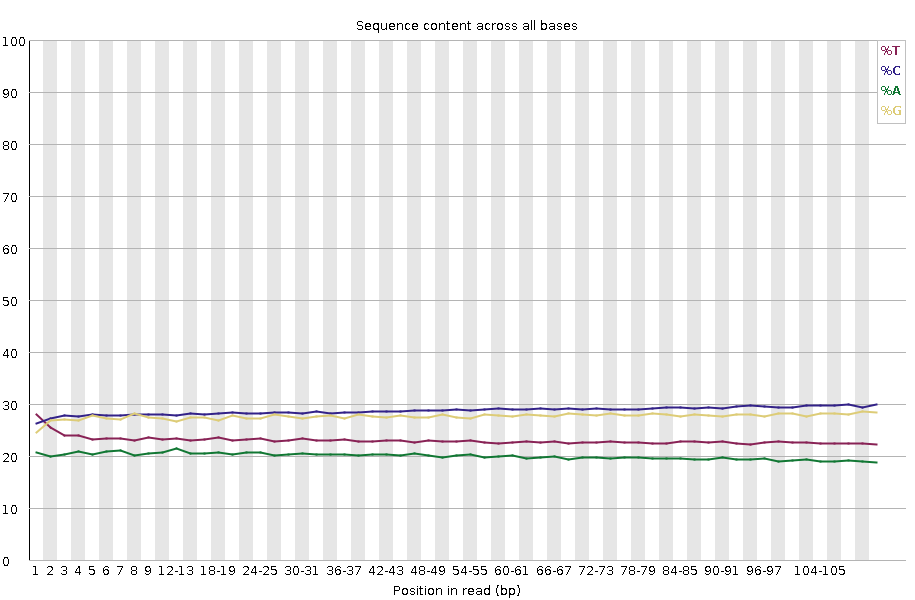
\includegraphics[width=\textwidth, height=4cm]{../../results/fastqc/Plot-Exports/fastqc_per_base_sequence_content_plot_CRR240976_f1_trim_p}
    \end{subfigure}
\end{figure}

\begin{figure}[htbp]
    \caption{FastQC quality assessment of the per base sequence quality of the raw FASTQ file CRR240976\_f1.fastq.gz vs the trimmed file CRR240976\_f1.trim.p.fastq.gz}
    \label{fig:0.1-FastQC-per_base_seq_qual-CRR240976-raw_vs_trim}
    \begin{subfigure}[t]{0.48\linewidth}
        \caption{Raw data}
        \label{fig:0.1-FastQC-per_base_seq_qual-CRR240976}
        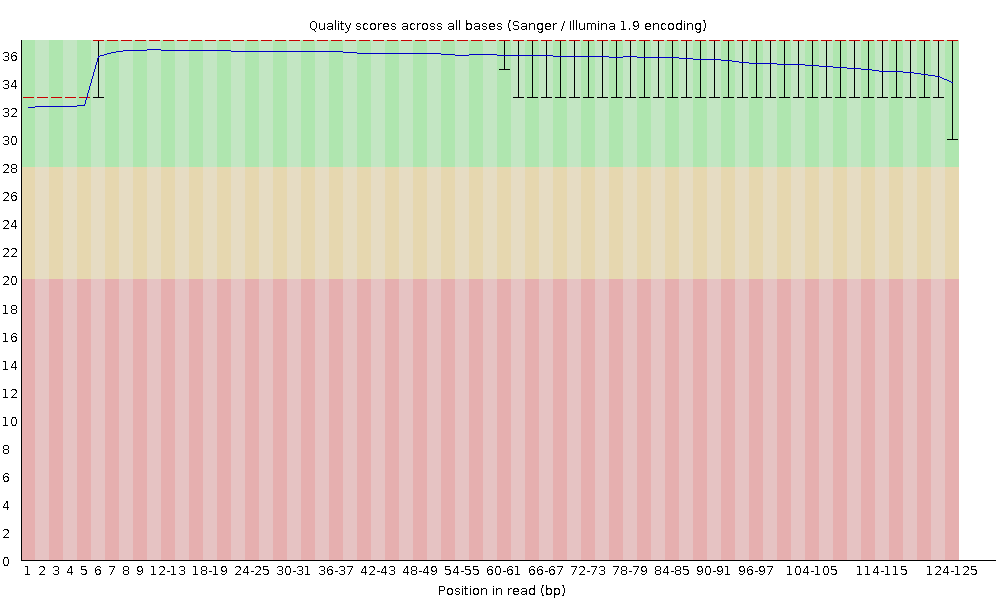
\includegraphics[width=\textwidth, height=4cm]{../../results/fastqc/Plot-Exports/fastqc_per_base_sequence_quality_plot_CRR240976_f1}
    \end{subfigure}
    \begin{subfigure}[t]{0.48\linewidth}
        \caption{Trimmed data}
        \label{fig:0.1-FastQC-per_base_seq_qual-CRR240976-trim}
        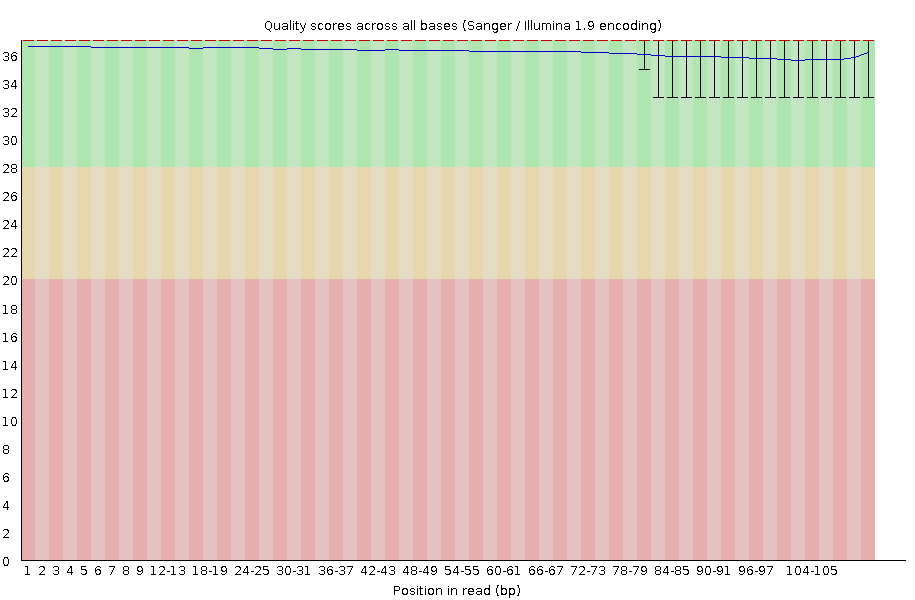
\includegraphics[width=\textwidth, height=4cm]{../../results/fastqc/Plot-Exports/fastqc_per_base_sequence_quality_plot_CRR240976_f1_trim_p}
    \end{subfigure}
\end{figure}


\subsection{Transcripts abundances quantification}

The mapping/pseudoalignment of the RNA-seq reads and the abundances quantification of the transcripts\index{transcript!abundances quantification} was done using kallisto\index{kallisto}. According to \autocite{10.1038/nbt.3519}, kallisto offers the following advantages over other alignment and quantification software:
\begin{quote}
    kallisto is a program for quantifying abundances of transcripts from RNA-Seq data, or more generally of target sequences using high-throughput sequencing reads. It is based on the novel idea of pseudoalignment for rapidly determining the compatibility of reads with targets, without the need for alignment. On benchmarks with standard RNA-Seq data, kallisto can quantify 30 million human bulk RNA-seq reads in less than 3 minutes on a Mac desktop computer using only the read sequences and a transcriptome index that itself takes than 10 minutes to build. Pseudoalignment of reads preserves the key information needed for quantification, and kallisto is therefore not only fast, but also comparably accurate to other existing quantification tools. In fact, because the pseudoalignment procedure is robust to errors in the reads, in many benchmarks kallisto significantly outperforms existing tools.
\end{quote}

kallisto requires a reference genome/transcriptome\index{genome/transcriptome!reference} for aligning the RNA-seq data. To this end, reference FASTA\index{FASTA} cDNA\index{DNA!cDNA} dumps of Oryza nivara, cultivar BJ278 and Oryza sativa, cultivar Nipponbare were downloaded from Ensembl\index{Ensembl}. The Ensembl project delivers reference data for genome interpretation for any species: genome assemblies from public archive are annotated with genes, regulatory regions, variants and comparative data to provide a foundation for scientific research and genome interpretation \autocite{10.1093/bioinformatics/btu170}.


\subsection{Statistical evaluation and differential expression analysis}

The preprocessed and aligned data was further evaluated and analyzed using an R-script\index{R} \autocite{R-base} executed within RStudio\index{R!RStudio} \autocite{RStudio}. The following sections describe the analysis steps in detail.

\subsubsection{Import of the kallisto transcript-level estimates}

The kallisto transcript-level estimates were imported using the R-package \verb|tximport|\index{R!package!tximport} \autocite{R-tximport, tximport2015}. Thereby, the  abundances, counts, and transcript lengths were summarized to the gene level.

Scaling method: average transcript length over samples and then the library size (parameter \verb|lengthScaledTPM|).

The mapping of the transcript IDs\index{transcript!ID} (used within the kallisto \verb|abundance.tsv| files) to the corresponding gene IDs\index{gene!ID} was done using the BioMart database \verb|plants_mart| hosted at \url{https://plants.ensembl.org}. Datasets: \verb|nivara_eg_gene| and \verb|osativa_eg_gene| for O. nivara and O. sativa, respectively. See \autocite{R-biomaRt, biomaRt2009}.

Figure \ref{fig:2.1-TPM-Stats} shows some basic transcripts per million (TPM\index{transcript!transcripts per million (TPM)}) statistics about the imported kallisto files.

\begin{figure}[htbp]
    \caption{TPM statistics about the imported kallisto data}
    \label{fig:2.1-TPM-Stats}
    \begin{subfigure}[t]{0.48\linewidth}
        \label{fig:2.1-TPM-Stats-Oryza_nivara}
        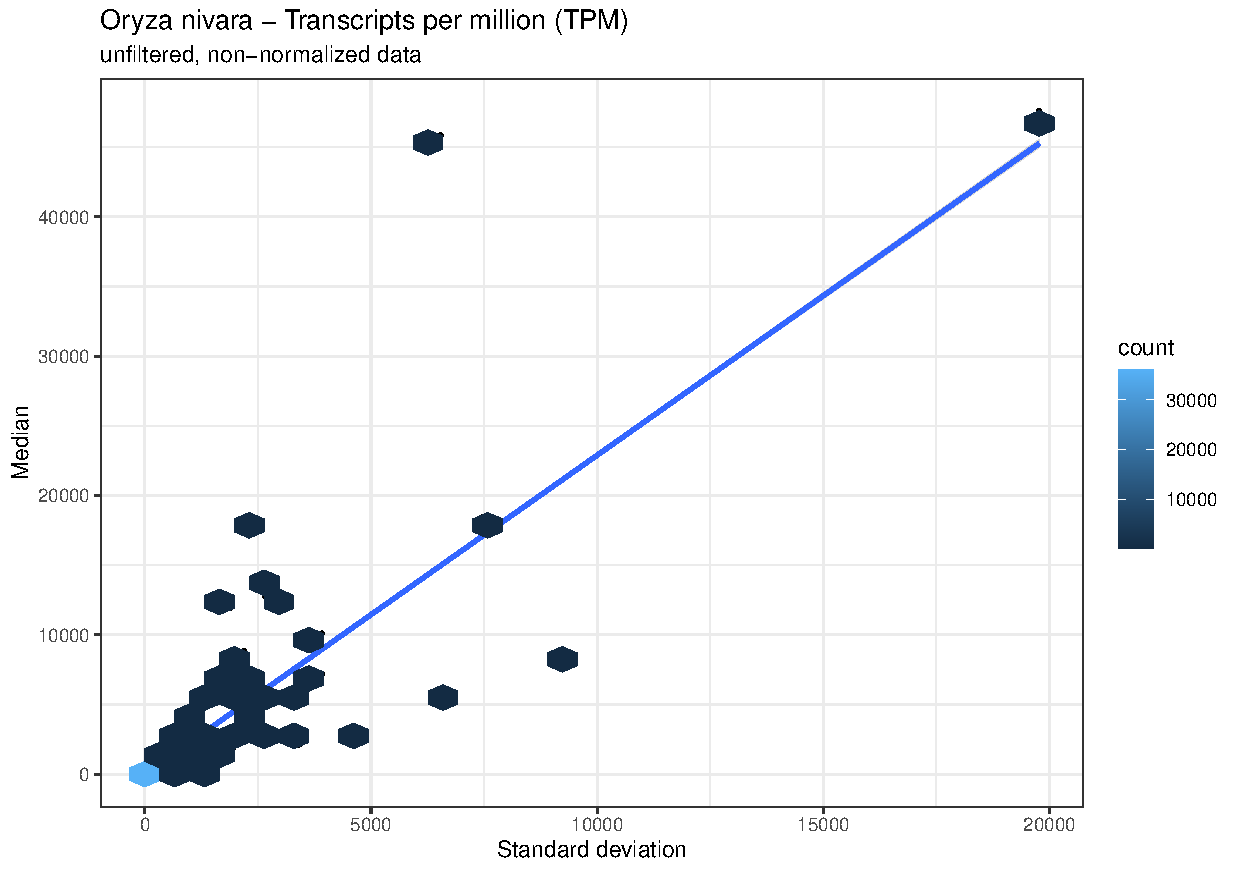
\includegraphics[width=\textwidth]{../../results/plots-and-tables/2.1-TPM-Stats-Oryza_nivara}
    \end{subfigure}
    \begin{subfigure}[t]{0.48\linewidth}
        \label{fig:2.1-TPM-Stats-Oryza_sativa}
        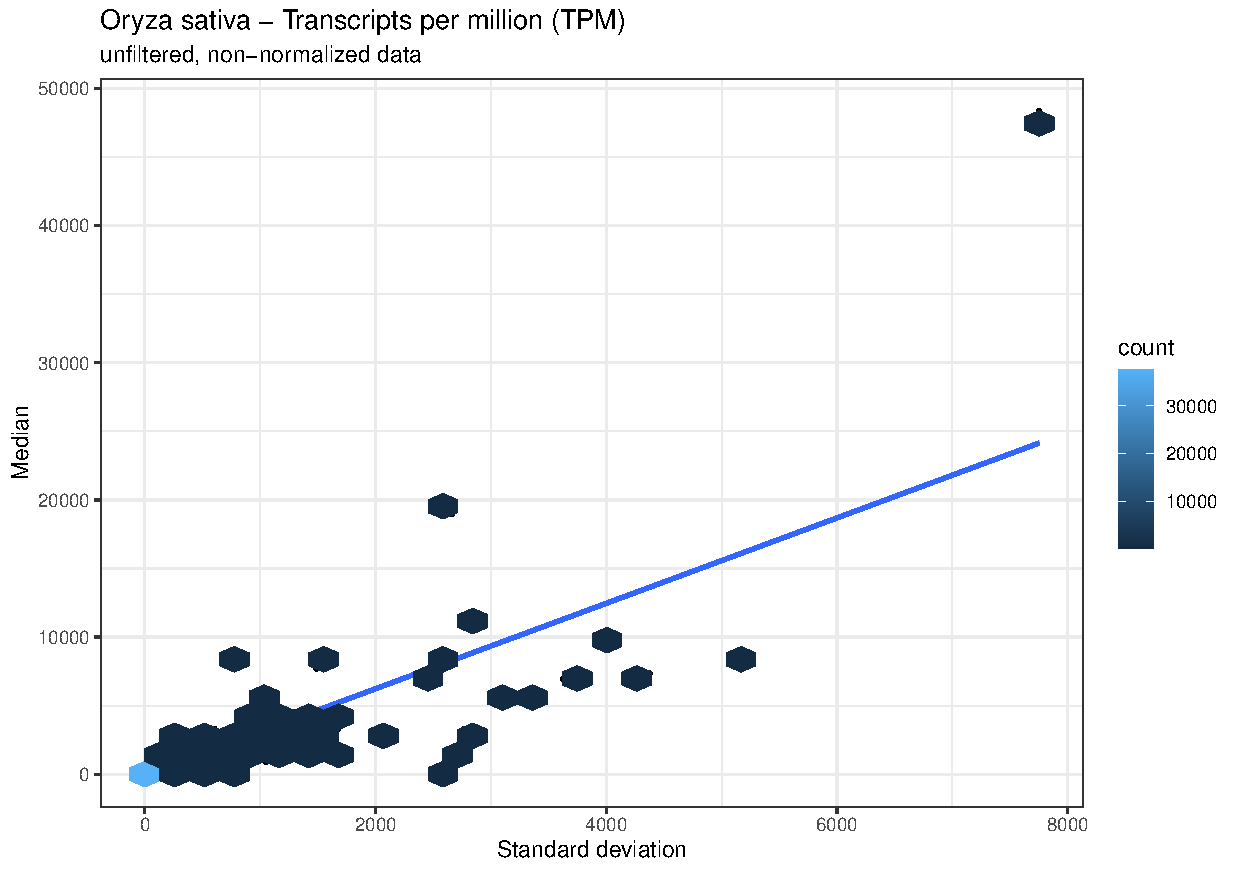
\includegraphics[width=\textwidth]{../../results/plots-and-tables/2.1-TPM-Stats-Oryza_sativa}
    \end{subfigure}
\end{figure}

\subsubsection{Filtering and normalization}

For further analysis, \verb|DGEList|-objects with counts per million (CPM)\index{counts per million (CPM)} and log2(CPM) values were created using the R-package \verb|edgeR|\index{R!package!edgeR} \autocite{R-edgeR, edgeR2010}. Figure \ref{fig:2.2-Log2CPM-unflt-notnorm} shows the distribution of the log2(CPM) values.

\begin{figure}[htbp]
    \caption{Log2(CPM) distribution of the unfiltered, non-normalized data}
    \label{fig:2.2-Log2CPM-unflt-notnorm}
    \begin{subfigure}[t]{0.64\linewidth}
        \label{fig:2.2-Log2CPM-unflt-notnorm-Oryza_nivara}
        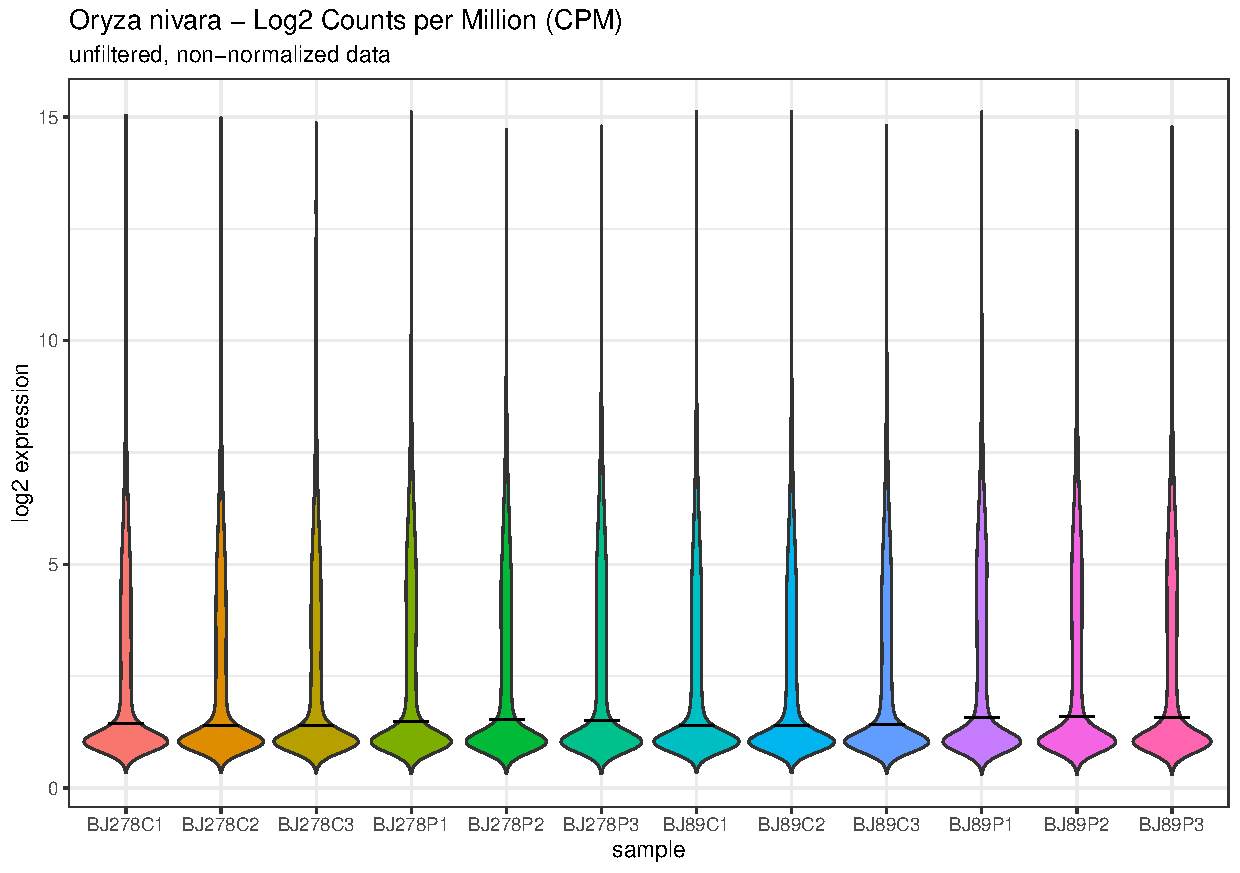
\includegraphics[width=\textwidth, height=4cm]{../../results/plots-and-tables/2.2-Log2CPM-unflt-notnorm-Oryza_nivara}
    \end{subfigure}
    \begin{subfigure}[t]{0.32\linewidth}
        \label{fig:2.2-Log2CPM-unflt-notnorm-Oryza_sativa}
        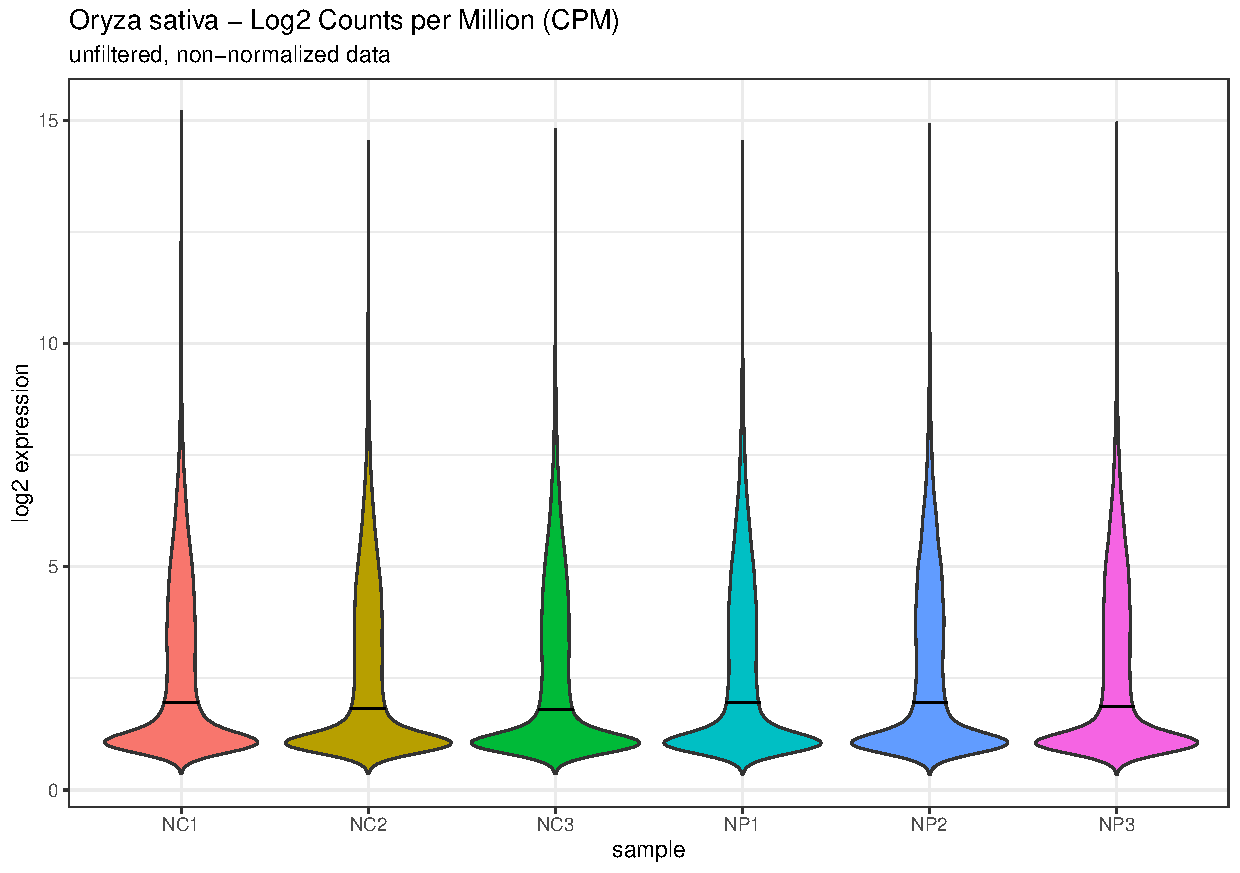
\includegraphics[width=\textwidth, height=4cm]{../../results/plots-and-tables/2.2-Log2CPM-unflt-notnorm-Oryza_sativa}
    \end{subfigure}
\end{figure}

In order to assess reasonable values for filtering the data, the number of genes with no reads at all (in none of the samples) and conversely the number of genes with CPMs \(\ge 1\) in at least 1, 2, 3, \dots\ of the samples were computed. Table \ref{tab:ufltr_cpm_stats} summarizes the results.

\begin{table}[htbp]
    \begin{threeparttable}
        \caption{Number of genes with no reads at all, and conversely number of genes with CPMs \(\ge 1\) in at least n = 1, 2, 3, \dots\ of the samples}
        \label{tab:ufltr_cpm_stats}
        \setlength\tabcolsep{6pt}
        \begin{tabular}{l l l p{30pt} p{30pt} p{30pt} p{30pt} p{30pt} p{30pt}}
            \toprule
                             &                  &                     & \multicolumn{6}{l}{Genes with CPMs \(\ge 1\) in at least n samples} \\
            \textbf{Species} & \(\Sigma\) genes & \(\Sigma\) no reads & 1     & 2     & 3     & 4     & 5     & 6     \\
            \midrule
            O. nivara        & 36313            & 7115                & 21001 & 20355 & 19891 & 19302 & 18895 & 18481 \\
            O. sativa        & 37967            & 4699                & 23934 & 22510 & 21609 & 20592 & 19715 & 18656 \\
            \bottomrule
        \end{tabular}
    \end{threeparttable}
\end{table}

Filtering out genes with low reads (\(< 1\) CPM in at least half of the samples) resulted in the distribution of the log2(CPM) values shown in figure \ref{fig:2.3-Log2CPM-flt-notnorm}.

\begin{figure}[htbp]
    \caption{Log2(CPM) distribution of the filtered (\(< 1\) CPM in at least half of the samples), non-normalized data}
    \label{fig:2.3-Log2CPM-flt-notnorm}
    \begin{subfigure}[t]{0.64\linewidth}
        \label{fig:2.3-Log2CPM-flt-notnorm-Oryza_nivara}
        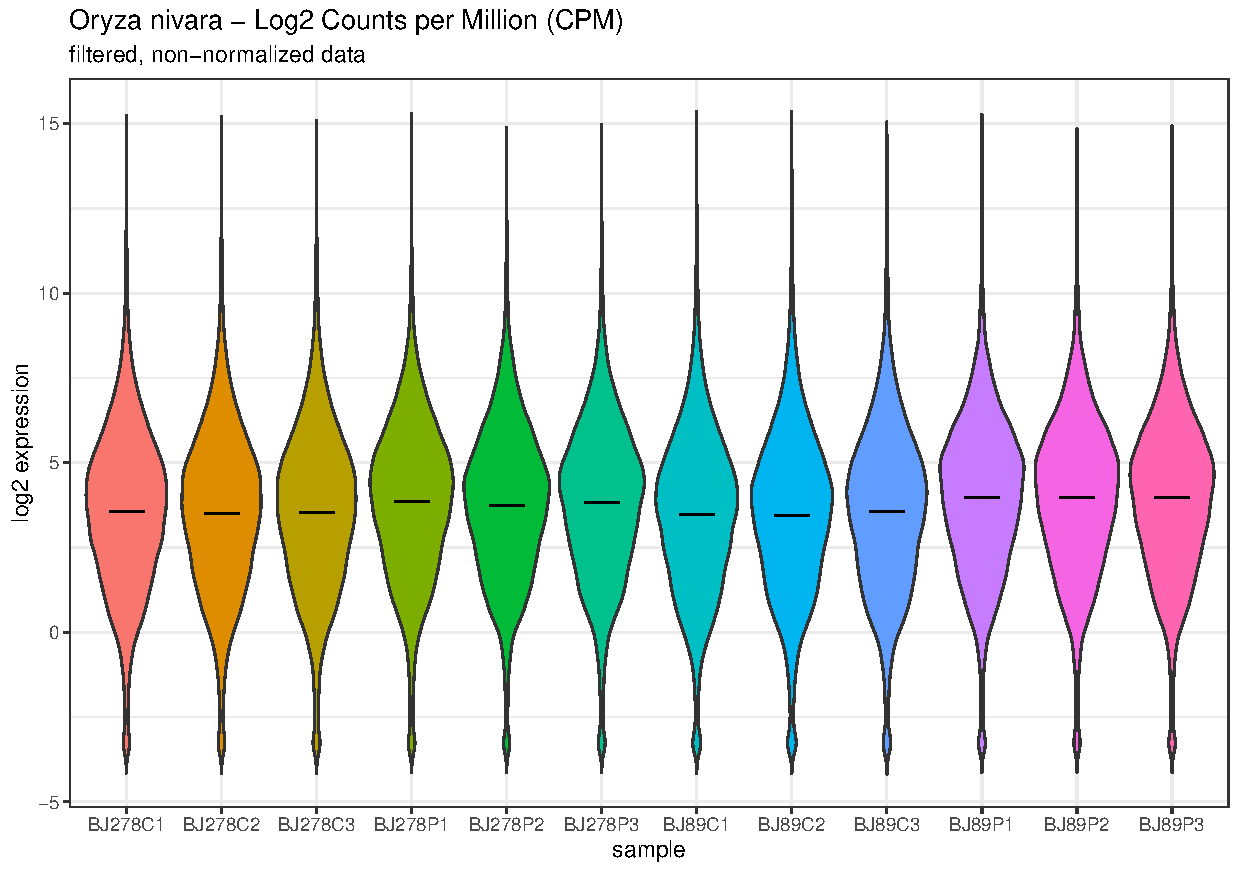
\includegraphics[width=\textwidth, height=4cm]{../../results/plots-and-tables/2.3-Log2CPM-flt-notnorm-Oryza_nivara}
    \end{subfigure}
    \begin{subfigure}[t]{0.32\linewidth}
        \label{fig:2.3-Log2CPM-flt-notnorm-Oryza_sativa}
        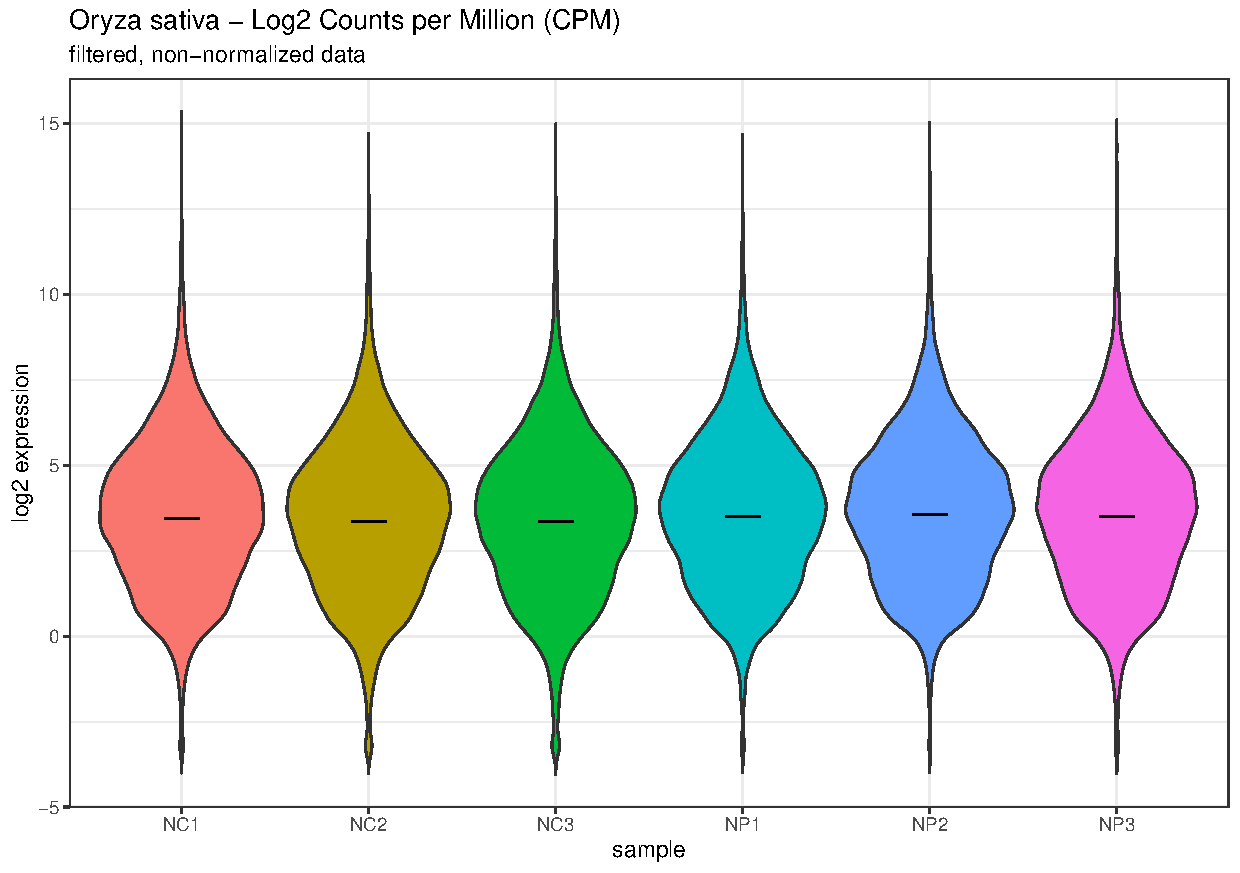
\includegraphics[width=\textwidth, height=4cm]{../../results/plots-and-tables/2.3-Log2CPM-flt-notnorm-Oryza_sativa}
    \end{subfigure}
\end{figure}

Finally, the filtered data was normalized using the \verb|edgeR| function \verb|calcNormFactors| which calculates scaling factors to convert raw library sizes into effective library sizes. Used normalization method: \verb|TMM|. The results of the normalization are shown in figure \ref{fig:2.4-Log2CPM-flt-norm}.

\begin{figure}[htbp]
    \caption{Log2(CPM) distribution of the filtered, normalized data}
    \label{fig:2.4-Log2CPM-flt-norm}
    \begin{subfigure}[t]{0.64\linewidth}
        \label{fig:2.4-Log2CPM-flt-norm-Oryza_nivara}
        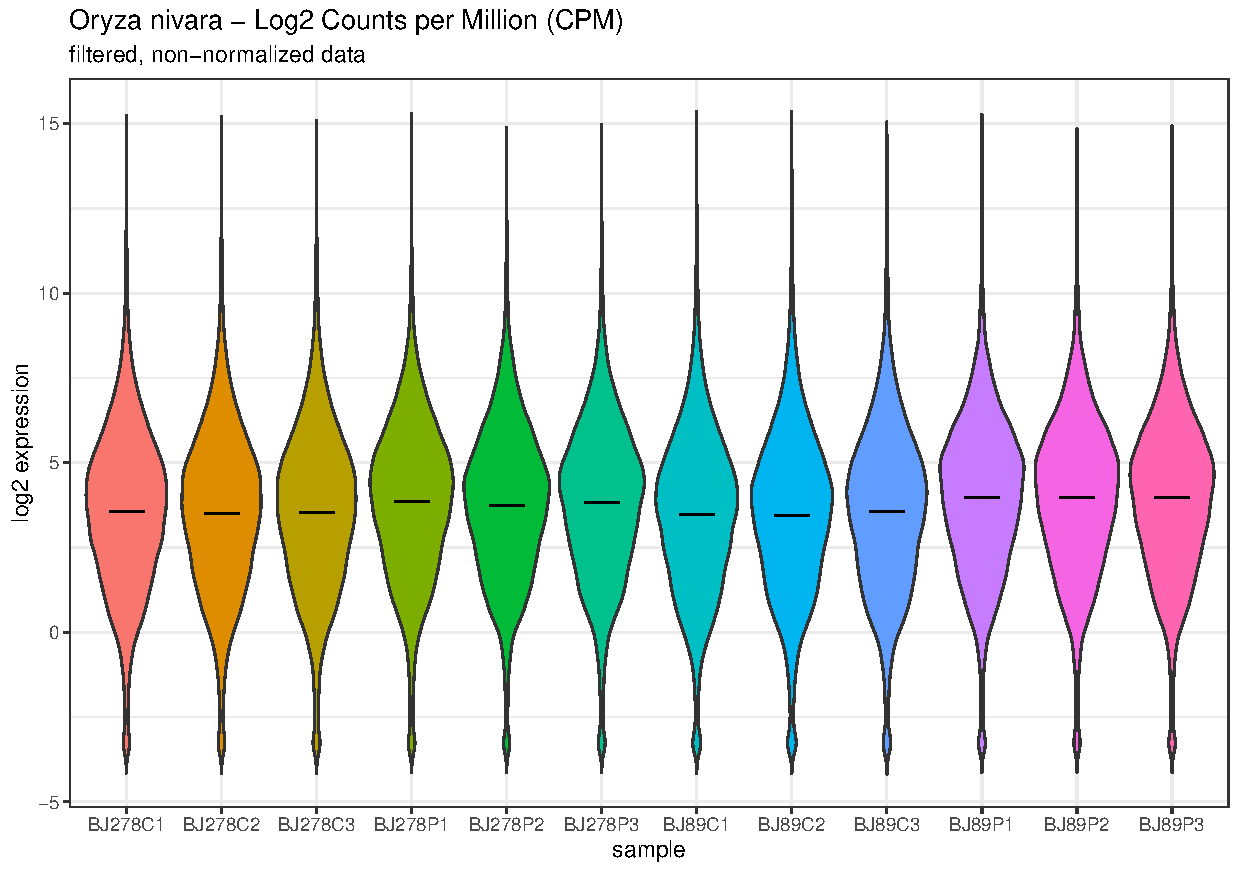
\includegraphics[width=\textwidth, height=4cm]{../../results/plots-and-tables/2.3-Log2CPM-flt-notnorm-Oryza_nivara}
    \end{subfigure}
    \begin{subfigure}[t]{0.32\linewidth}
        \label{fig:2.4-Log2CPM-flt-norm-Oryza_sativa}
        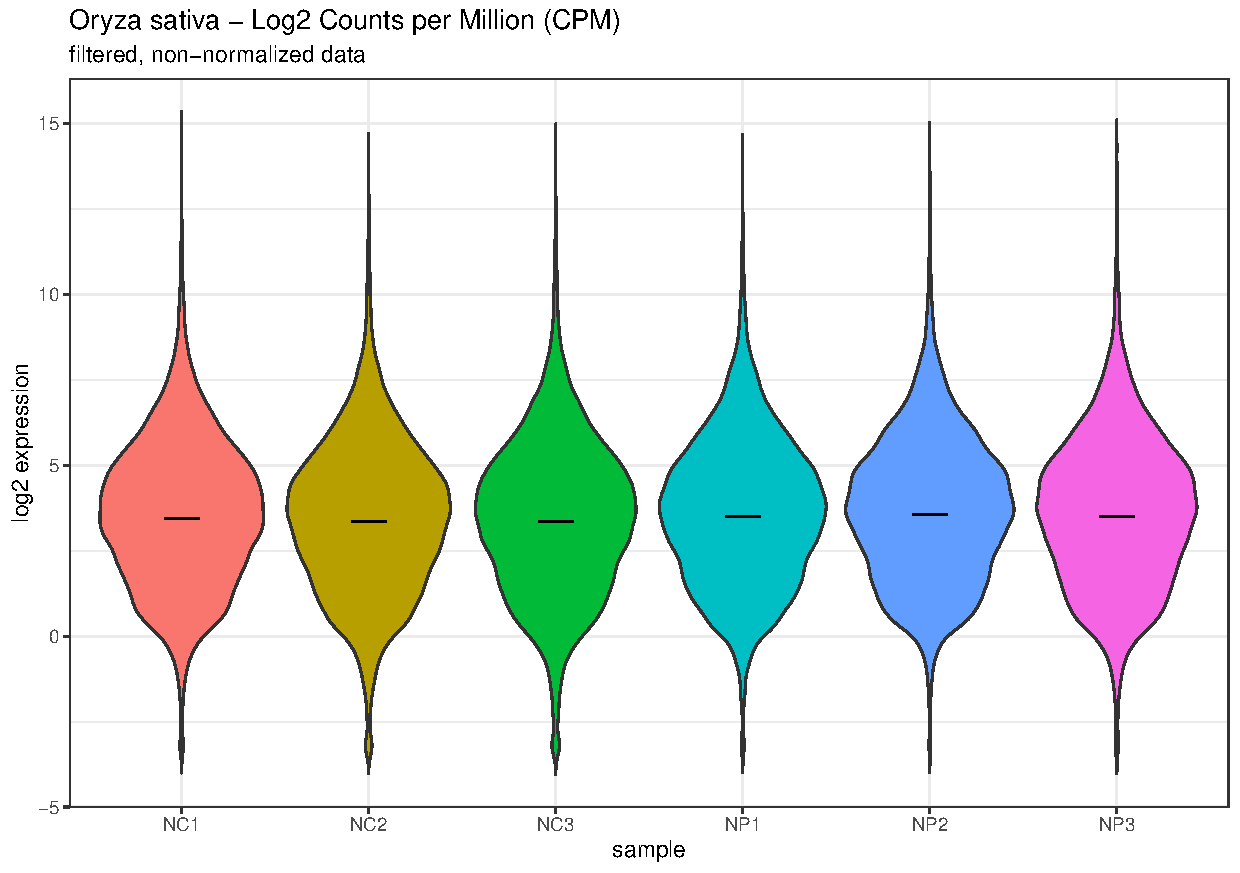
\includegraphics[width=\textwidth, height=4cm]{../../results/plots-and-tables/2.3-Log2CPM-flt-notnorm-Oryza_sativa}
    \end{subfigure}
\end{figure}

Figure \ref{fig:2.5-Log2CPM-Overview} provides an overview of the filtering and normalization results.

\begin{figure}[htbp]
    \caption{Log2(CPM) distribution of the filtered, normalized data in comparison with the non-normalized and the unfiltered data}
    \label{fig:2.5-Log2CPM-Overview}
    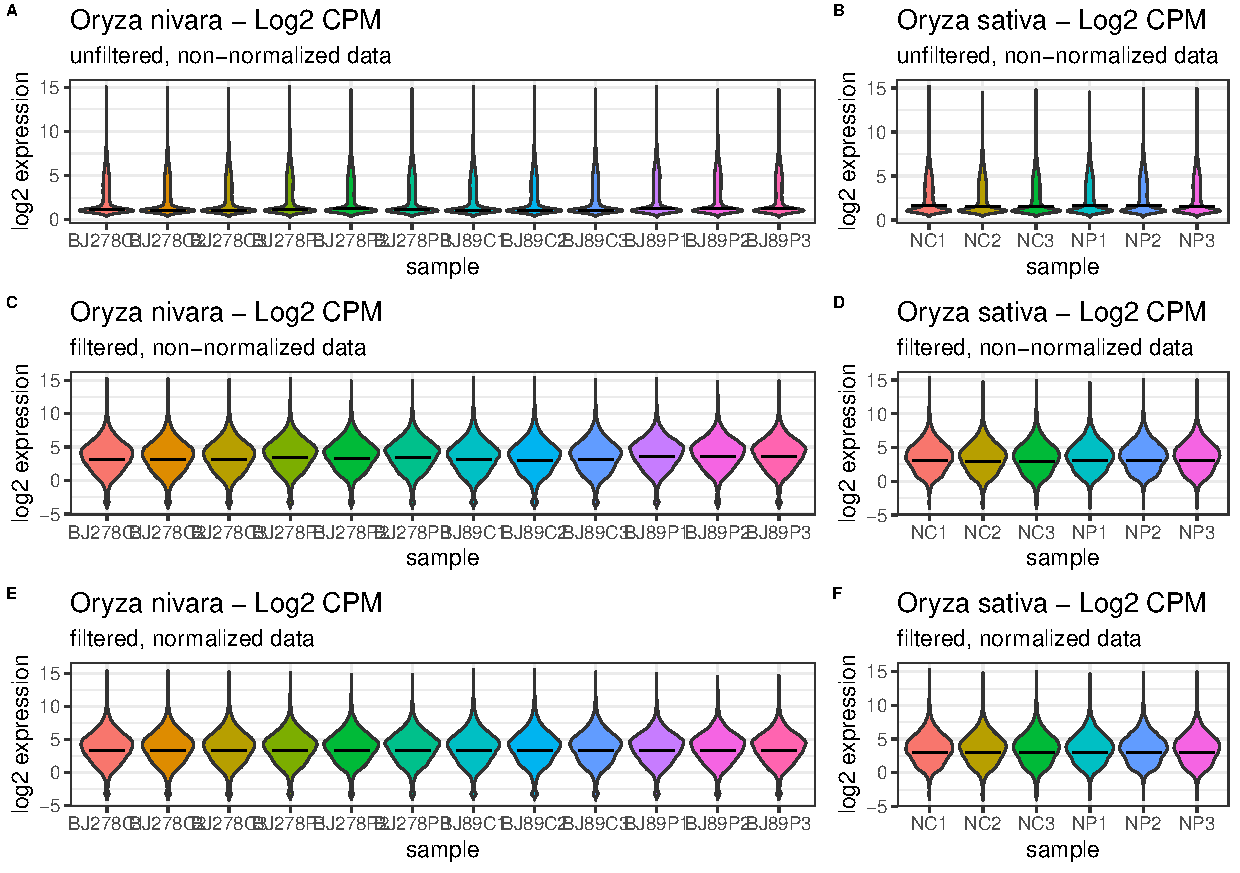
\includegraphics[width=\textwidth]{../../results/plots-and-tables/2.5-Log2CPM-Overview}
\end{figure}

\subsubsection{Hierarchical cluster analysis}

A hierarchical cluster analysis (HCA)\index{hierarchical cluster analysis (HCA)} was performed via the \verb|stats|\index{R!package!stats} function \verb|hclust| on the Euclidean distance matrix\index{hierarchical cluster analysis (HCA)!Euclidean distance matrix} of the log2(CPM) values. Used agglomeration method: \verb|method = complete|.

\subsubsection{Principal component analysis}

A principal component analysis (PCA)\index{principal component analysis (PCA)} was performed via the \verb|stats|\index{R!package!stats} function \verb|prcomp|.

\subsubsection{Identification of differentially expressed genes}

In order to identify differentially expressed genes (DEGs)\index{differentially expressed genes (DEGs)}, design and contrast matrices were created using the \verb|stats|\index{R!package!stats} function \verb|model.matrix| and the \verb|limma|\index{R!package!limma} function \verb|makeContrasts|.

The design matrices were used to create linear model fits for each gene via the \verb|limma|\index{R!package!limma} functions \verb|voom| and \verb|lmFit|.

The linear model fits and the contrast matrices were used to calculate estimated coefficients and standard errors (contrasts) via the \verb|limma|\index{R!package!limma} function \verb|contrasts.fit|.

The contrasts were used to "calculate moderated t-statistics, moderated F-statistic, and log-odds of differential expression by empirical Bayes moderation of the standard errors towards a global value" (empirical Bayes statistics) via the \verb|limma|\index{R!package!limma} function \verb|eBayes| \autocite{R-limma}.

Finally, the empirical Bayes statistics were used to extract a table of the top-ranked genes via the \verb|limma|\index{R!package!limma} function \verb|topTable| (sorted by the \verb|LogFC|\index{LogFC}-values).

Venn diagrams of the DEGs (according to the calculated empirical Bayes statistics) were created via the \verb|gprofiler2|\index{R!package!gprofiler2} function \verb|decideTests| (with parameters \verb|method = "global"|, \verb|adjust.method = "BH"|, \verb|p.value = 0.01|, \verb|lfc = 7|) and the \verb|limma| function \verb|vennDiagram|.

See \autocite{limma2015} for details on the statistical foundations implemented by \verb|limma|\index{R!package!limma}.

\subsection{Functional enrichment analysis}

A functional enrichment analysis of the 100 "top-ranked" genes was performed via the \verb|gprofiler2|\index{R!package!gprofiler2} function \verb|gost| (with \verb|correction_method = "fdr"| \autocite{R-gprofiler2}.

    \section{Results}

\subsection{Quality evaluation}

The RNA-seq data was initially assessed with FastQC\index{FastQC}, and according to this assessment the data was preprocessed/trimmed with Trimmomatic\index{Trimmomatic} and afterwards assessed again with FastQC. Finally, an overall report on the data preprocessing, the quality assessments and the kallisto\index{kallisto} pseudoalignments was created with MultiQC\index{MultiQC}.

Figure \ref{fig:0.1-MultiQC_FastQC_status_checks} shows the MultiQC report on the Trimmomatic\index{Trimmomatic} preprocessing (the surviving reads).

\begin{figure}[htbp]
    \caption{Trimmomatic preprocessing}
    \label{fig:0.1-MultiQC_FastQC_status_checks}
    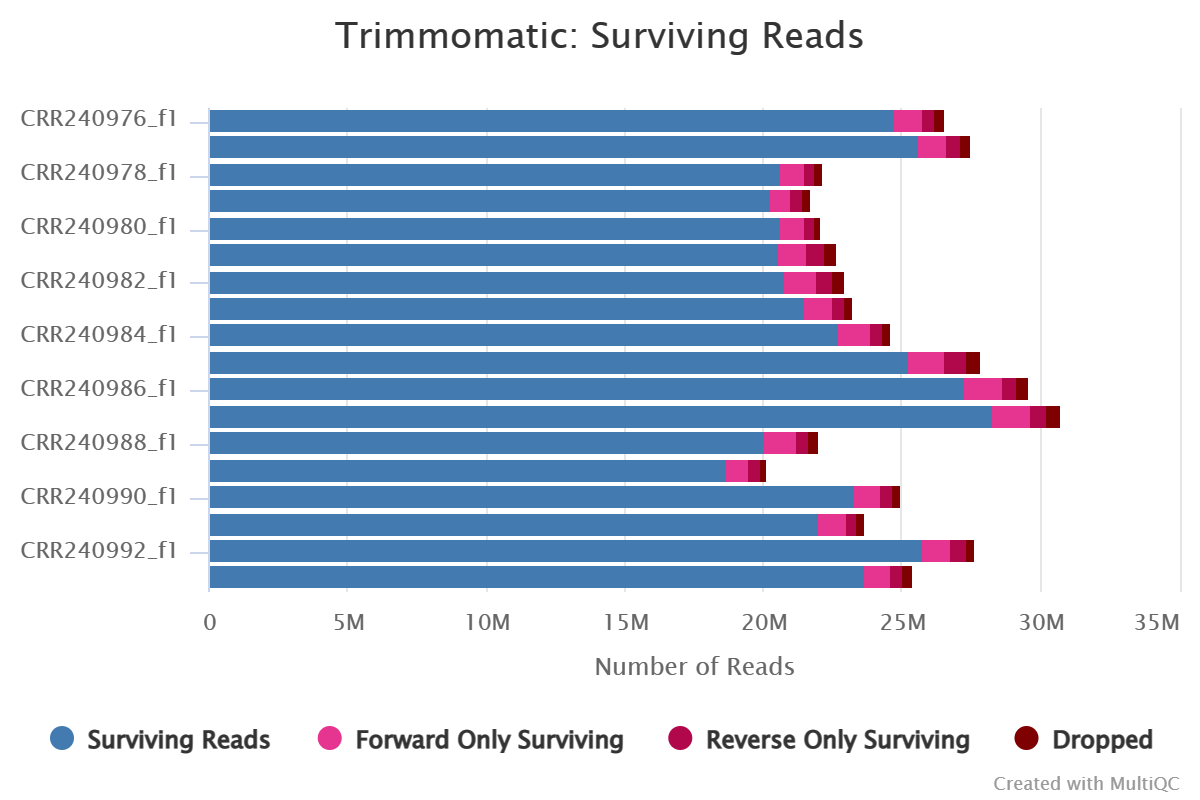
\includegraphics[width=0.9\textwidth]{../../results/multiqc/Plot-Exports/trimmomatic-surviving_reads}
\end{figure}

Figure \ref{fig:0.2-MultiQC_FastQC_status_checks} shows the MultiQC overview of the FastQC\index{FastQC} quality assessments of the trimmed FASTQ files.

\begin{figure}[htbp]
    \caption{FastQC quality assessment of the preprocessed FASTQ files}
    \label{fig:0.2-MultiQC_FastQC_status_checks}
    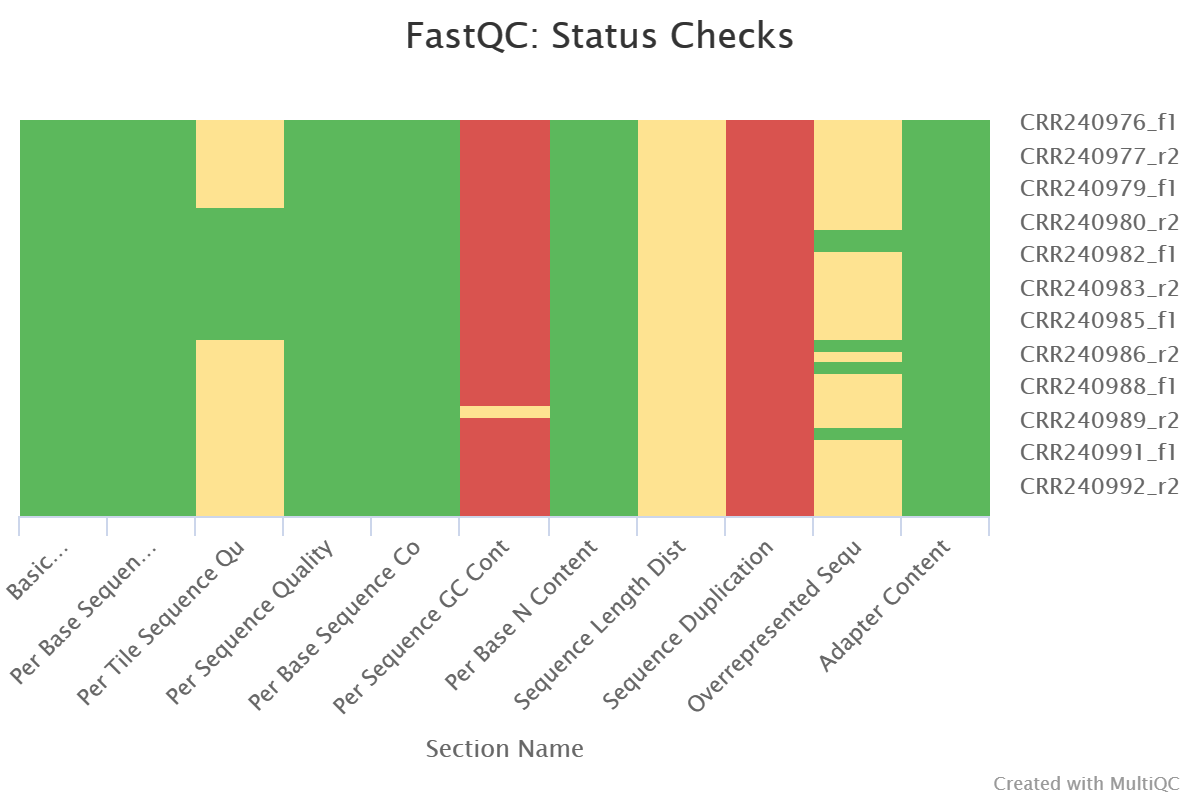
\includegraphics[width=0.9\textwidth]{../../results/multiqc/Plot-Exports/fastqc-status-check-heatmap}
\end{figure}

According to these quality assessments, the (trimmed) RNA-seq data may be regarded as good quality for the purpose of this research.


\subsection{Reads mapped to the reference transcriptome}

For most of the FASTQ files, kallisto pseudoaligned well above 80 \% of the (preprocessed) RNA-seq reads. Figure \ref{fig:0.3-MultiQC_kallisto_alignment} shows a MultiQC overview of the kallisto\index{kallisto} pseudoalignments.

\begin{figure}[htbp]
    \caption{kallisto pseudoalignments}
    \label{fig:0.3-MultiQC_kallisto_alignment}
    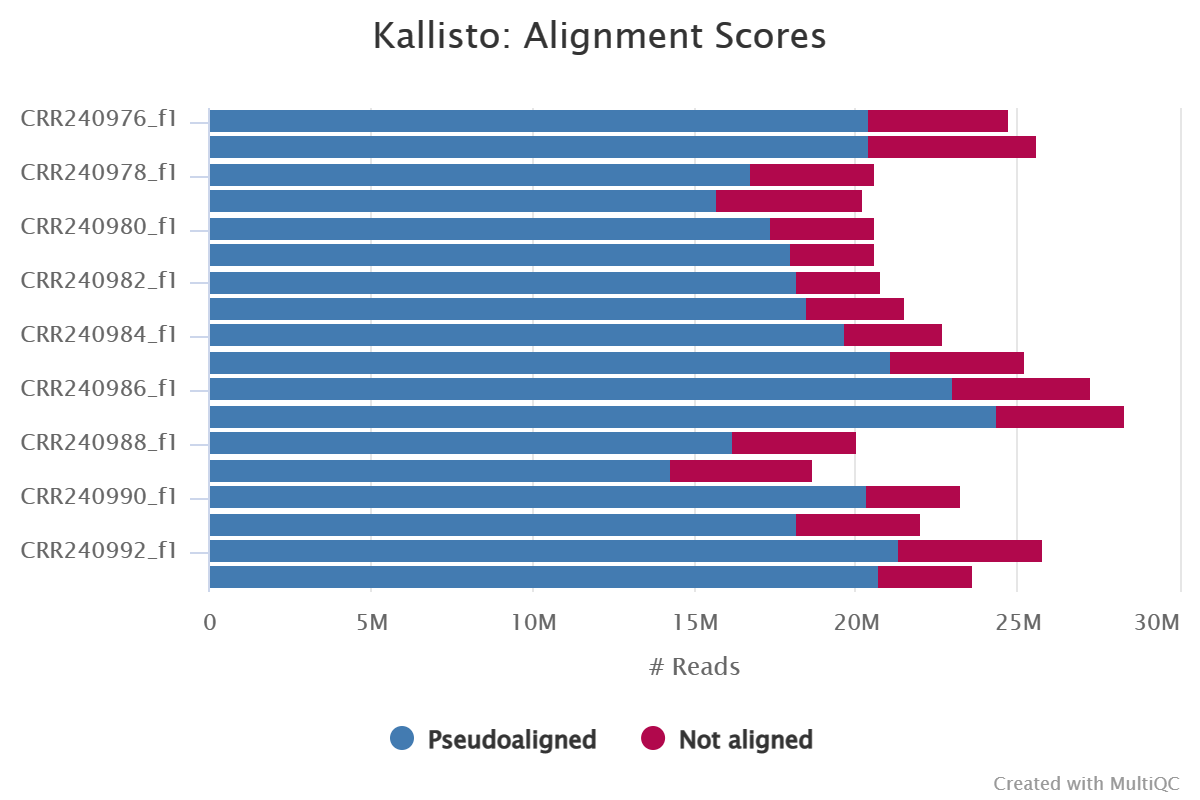
\includegraphics[width=0.9\textwidth]{../../results/multiqc/Plot-Exports/kallisto_alignment}
\end{figure}


\subsection{Hierarchical cluster analysis}

The hierarchical cluster analysis\index{hierarchical cluster analysis (HCA)} reveals that the normal condition groups and the drought stress condition groups are closely related (grouped together). But the data for O. nivara also shows that the cultivar has an even greater impact on the clustering then the drought stress condition (see figures \ref{fig:3.1-Clust-Dendrogram-Oryza_nivara} and \ref{fig:3.1-Clust-Dendrogram-Oryza_sativa}).

\begin{figure}[htbp]
    \caption{Hierarchical cluster analysis of the O. nivara RNA-seq data}
    \label{fig:3.1-Clust-Dendrogram-Oryza_nivara}
    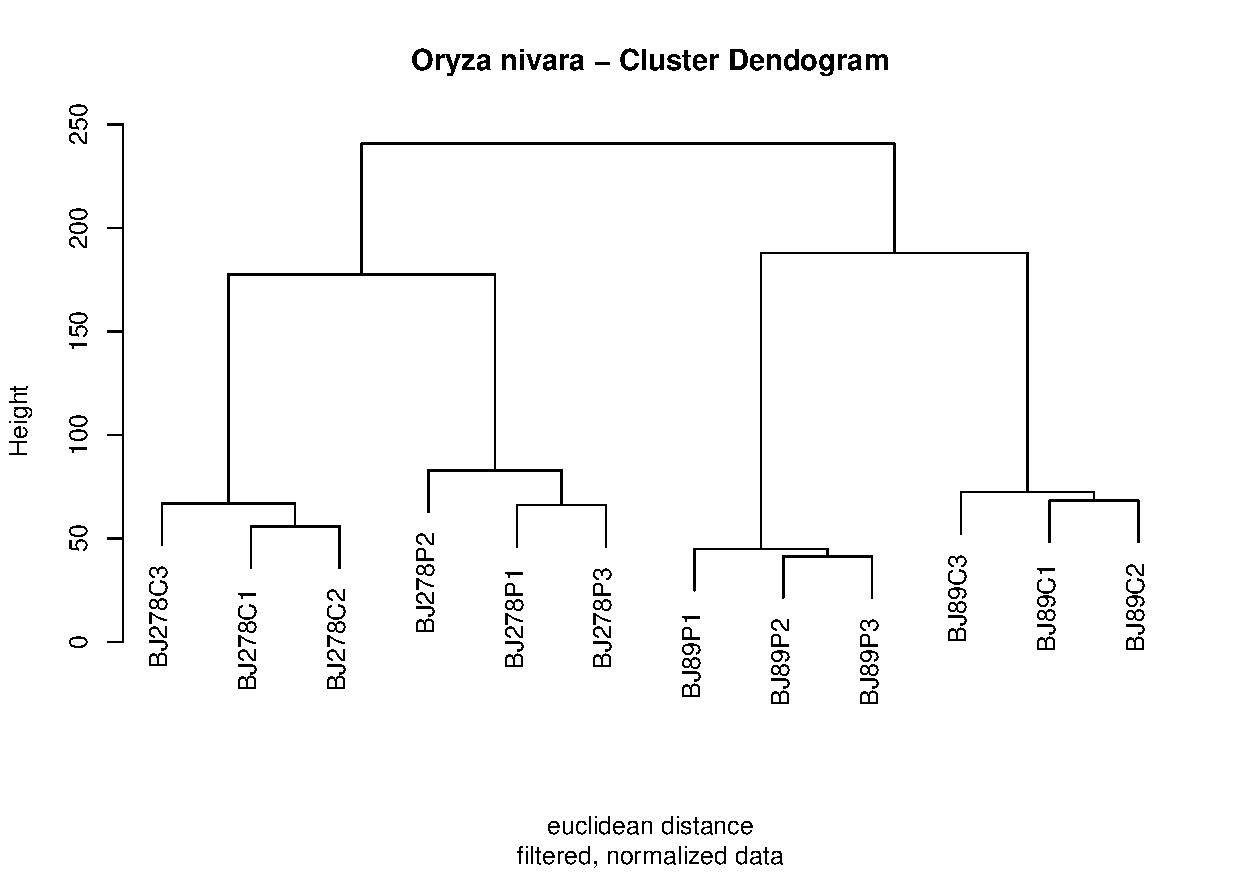
\includegraphics[width=0.9\textwidth]{../../results/plots-and-tables/3.1-Clust-Dendrogram-Oryza_nivara}
\end{figure}

\begin{figure}[htbp]
    \caption{Hierarchical cluster analysis of the O. sativa RNA-seq data}
    \label{fig:3.1-Clust-Dendrogram-Oryza_sativa}
    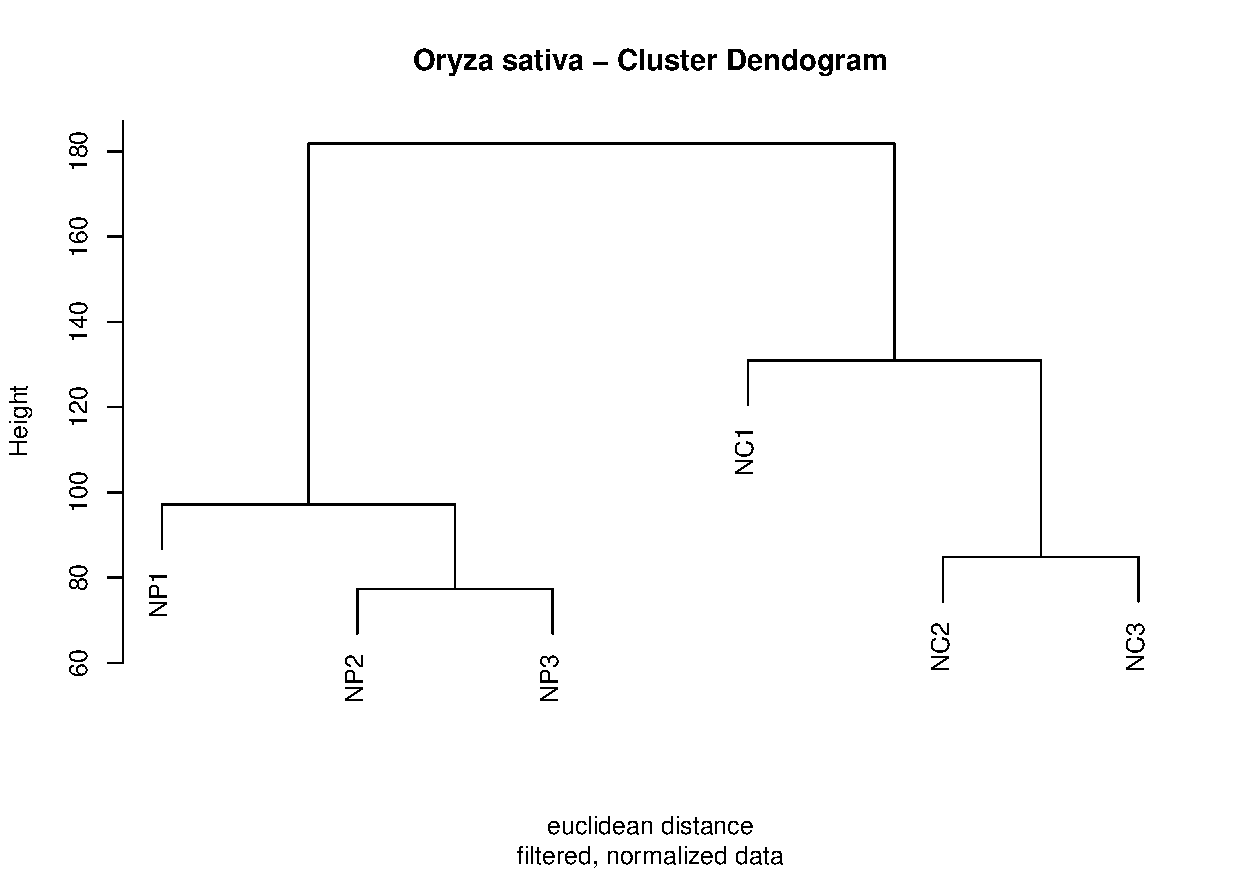
\includegraphics[width=0.9\textwidth]{../../results/plots-and-tables/3.1-Clust-Dendrogram-Oryza_sativa}
\end{figure}


\subsection{Principal component analysis}

The principal component analysis (PCA)\index{principal component analysis (PCA)} reveals that for both O. nivara and O. sativa the first two principal components account for more than 80 \% of the variance in the gene expression. Figures  \ref{fig:3.2-PCA-Oryza_nivara} and \ref{fig:3.2-PCA-Oryza_sativa} show the contribution percentage of the samples to the first two principal components (PCs)\index{principal component analysis (PCA)!principal component (PC)} for the two species.

For O. nivara, the samples from the same condition (normal vs drought stress) cluster together, with a tight clustering of the two different cultivars. This means that the different conditions might well explain the differences in gene expression, with the cultivar being an important confounding factor.

For O. sativa, the samples from the same condition cluster together with the exception of sample "NC1". This might be due to a batch effect\index{batch effect}.

\begin{figure}[htbp]
    \caption{PCA of the log2(CPM) data - O. nivara}
    \label{fig:3.2-PCA-Oryza_nivara}
    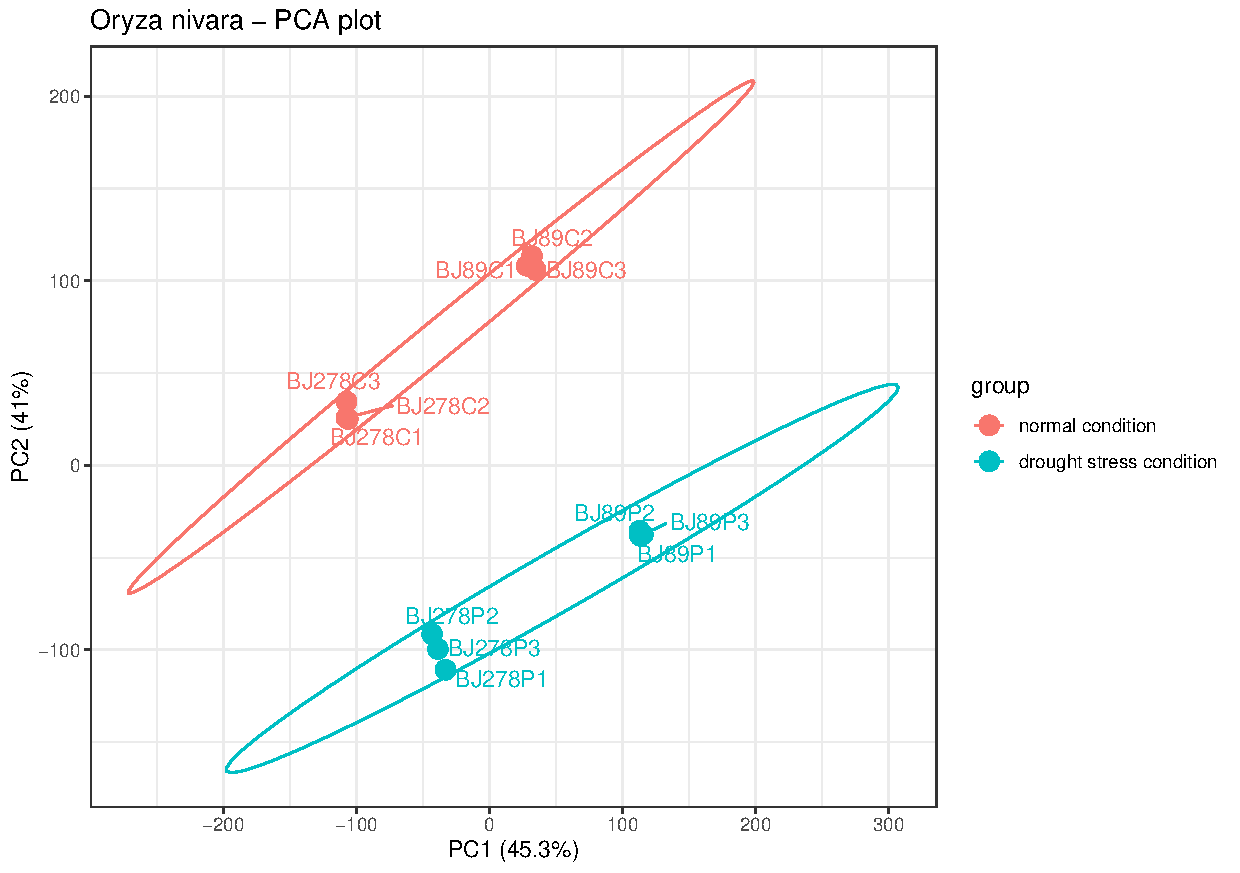
\includegraphics[width=0.9\textwidth]{../../results/plots-and-tables/3.2-PCA-Oryza_nivara}
\end{figure}

\begin{figure}[htbp]
    \caption{PCA of the log2(CPM) data - O. sativa}
    \label{fig:3.2-PCA-Oryza_sativa}
    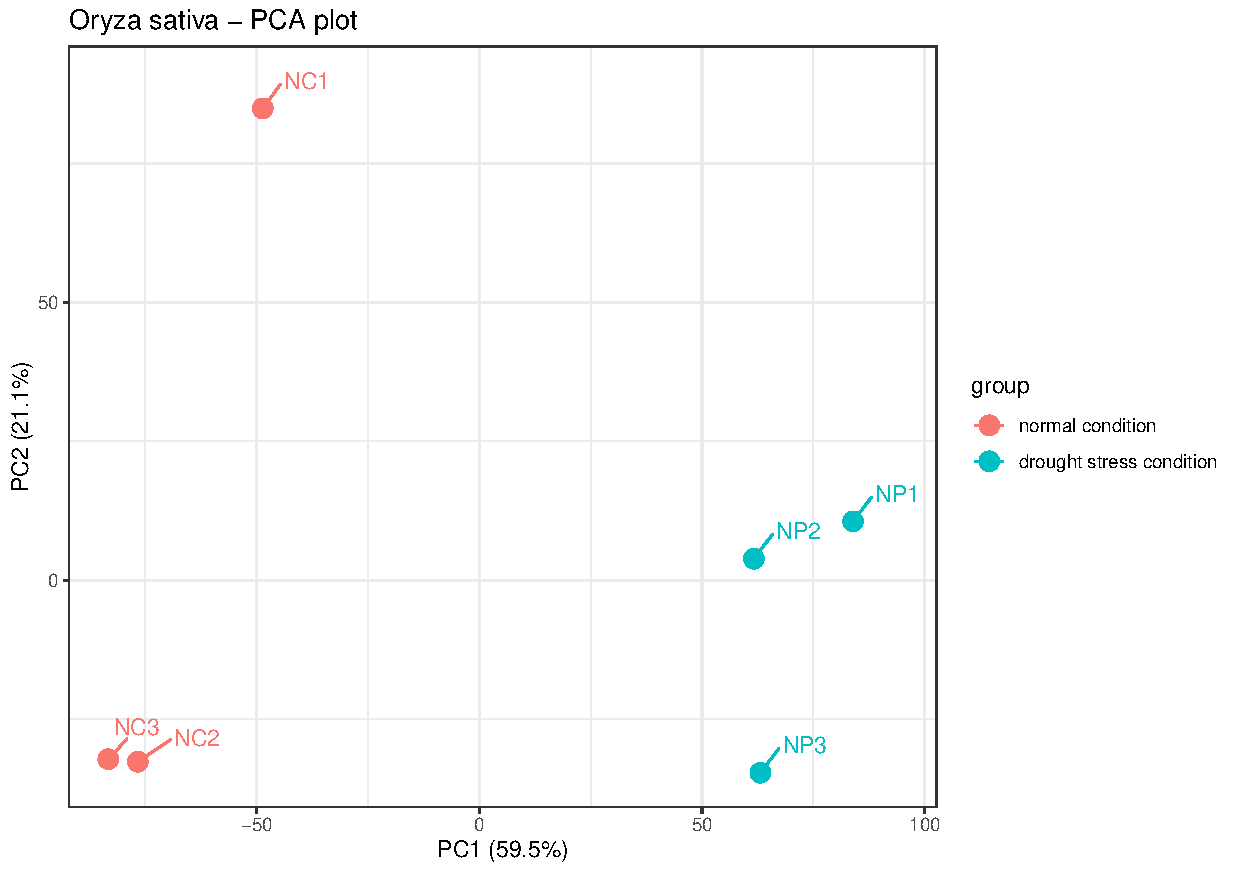
\includegraphics[width=0.9\textwidth]{../../results/plots-and-tables/3.2-PCA-Oryza_sativa}
\end{figure}


\subsection{Differentially expressed genes}

The volcano plots \ref{fig:4.1-DEG-Volcano-Plot-Oryza_nivara} and \ref{fig:4.1-DEG-Volcano-Plot-Oryza_sativa} provide a quick overview of the genes with large fold changes that are also statistically significant. These may be the biologically most significant genes.

\begin{figure}[htbp]
    \caption{Volcano plot of the DEGs - O. nivara}
    \label{fig:4.1-DEG-Volcano-Plot-Oryza_nivara}
    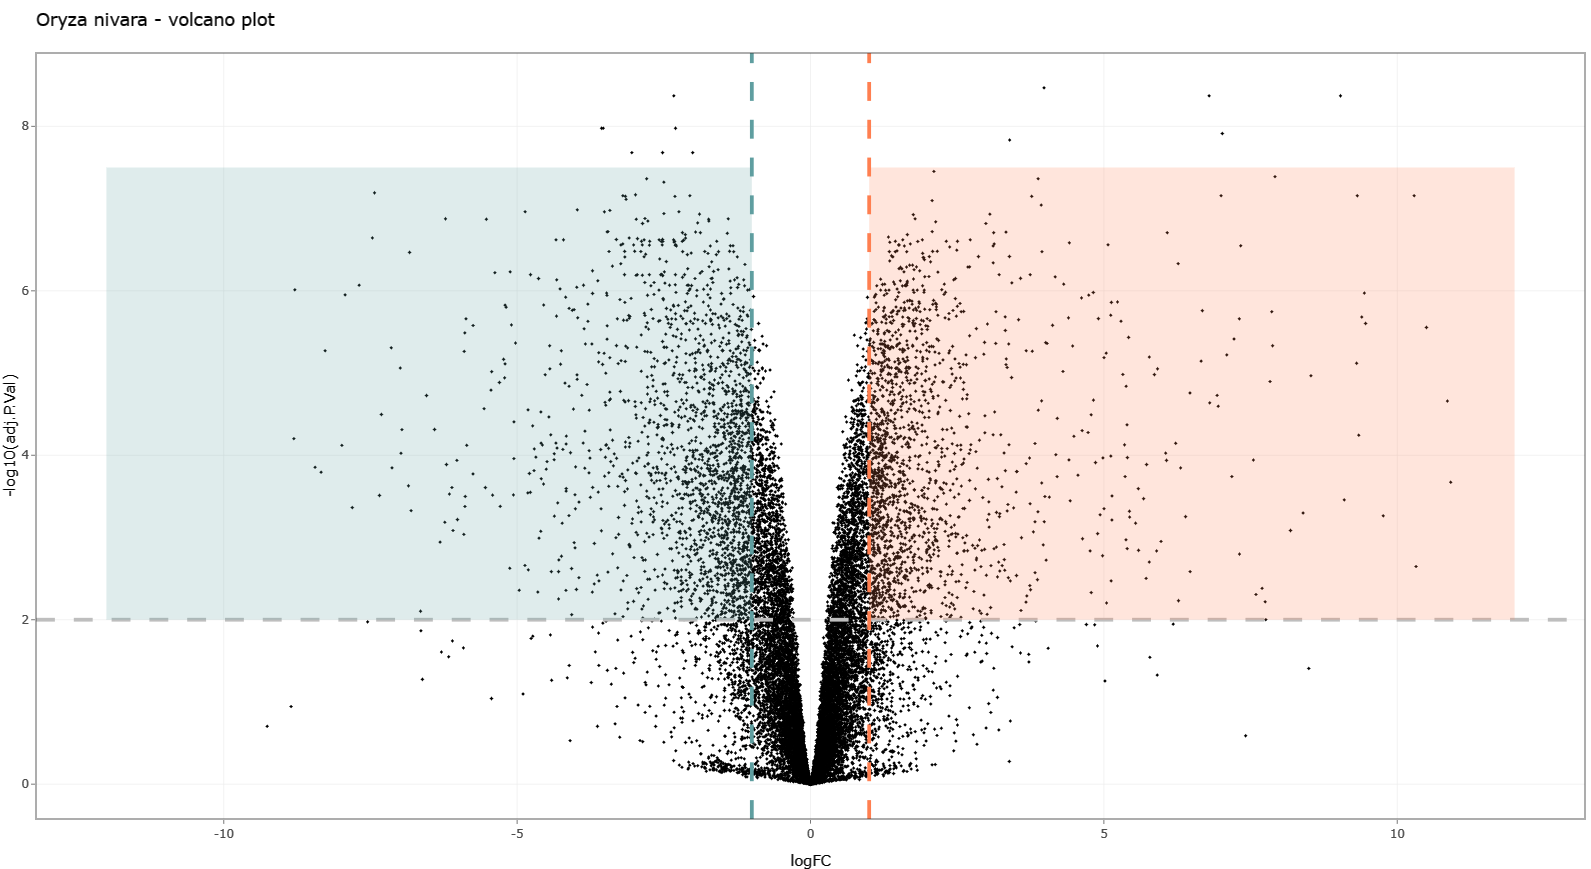
\includegraphics[width=0.9\textwidth]{../../results/plots-and-tables/4.1-DEG-Volcano-Plot-Oryza_nivara}
\end{figure}

\begin{figure}[htbp]
    \caption{Volcano plot of the DEGs - O. sativa}
    \label{fig:4.1-DEG-Volcano-Plot-Oryza_sativa}
    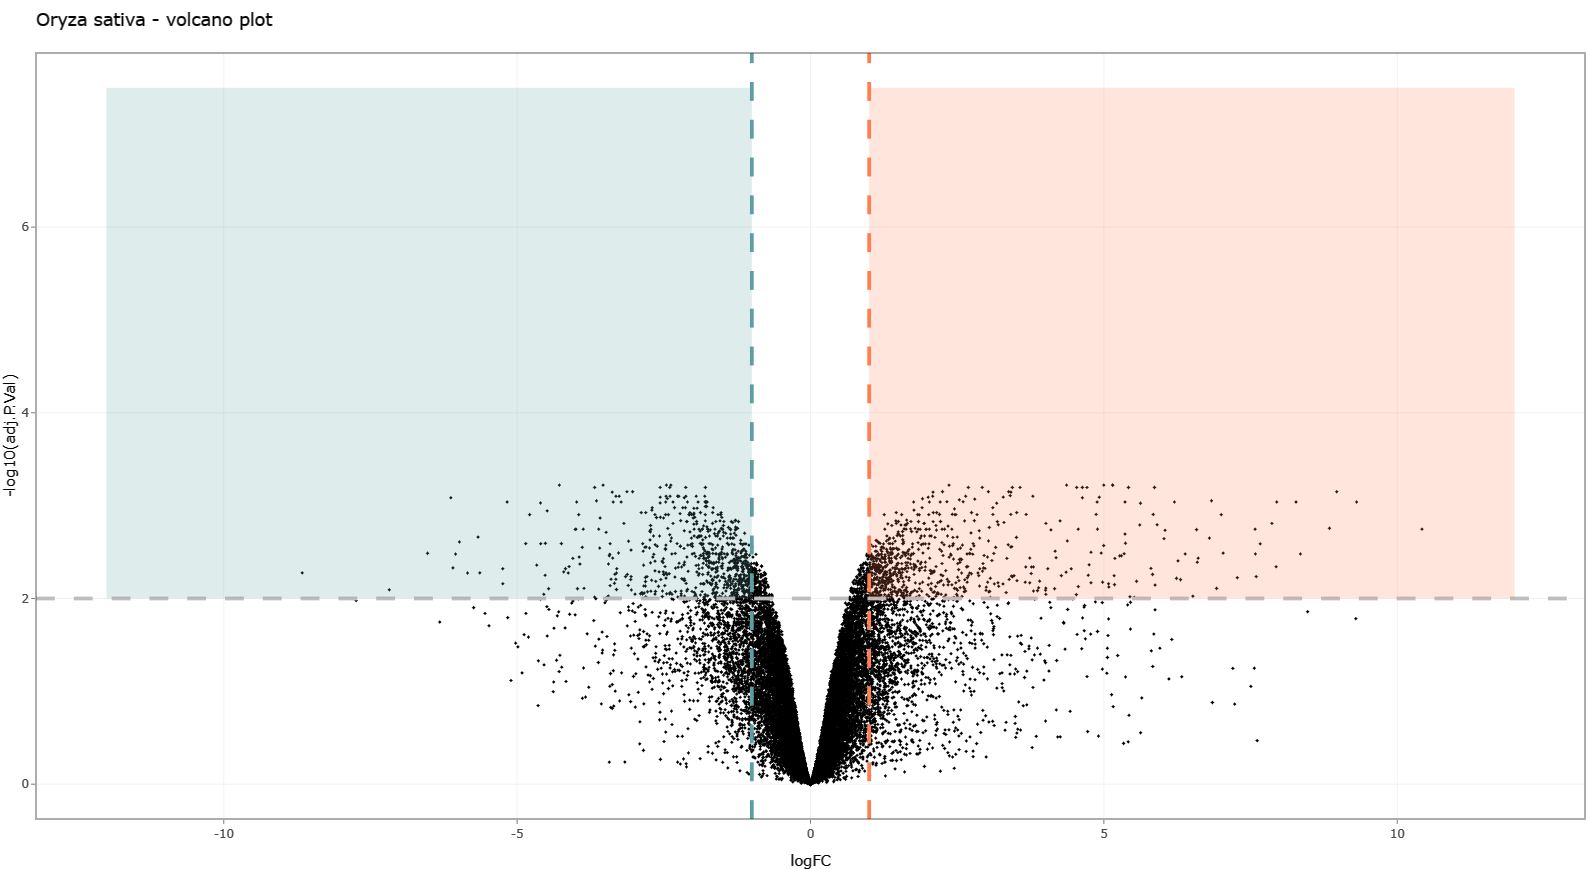
\includegraphics[width=0.9\textwidth]{../../results/plots-and-tables/4.1-DEG-Volcano-Plot-Oryza_sativa}
\end{figure}

According to the limma tests with a p-value of one percent, there are 15 down- vs 33 up-regulated genes for O. nivara under drought stress conditions, and 2 down- vs 16 up-regulated for O. sativa. Figure \ref{fig:4.2-DEG-Venn-Diagr} shows the respective Venn diagrams. Figures \ref{fig:4.4-DEG-Heatmap-Oryza_nivara} and \ref{fig:4.4-DEG-Heatmap-Oryza_sativa} present heatmaps of these genes.

\begin{figure}[htbp]
    \caption{Venn diagrams of the DEGs}
    \label{fig:4.2-DEG-Venn-Diagr}
    \begin{subfigure}[t]{0.44\linewidth}
        \caption{O. nivara}
        \label{fig:4.2-DEG-Venn-Diagr-Oryza_nivara}
        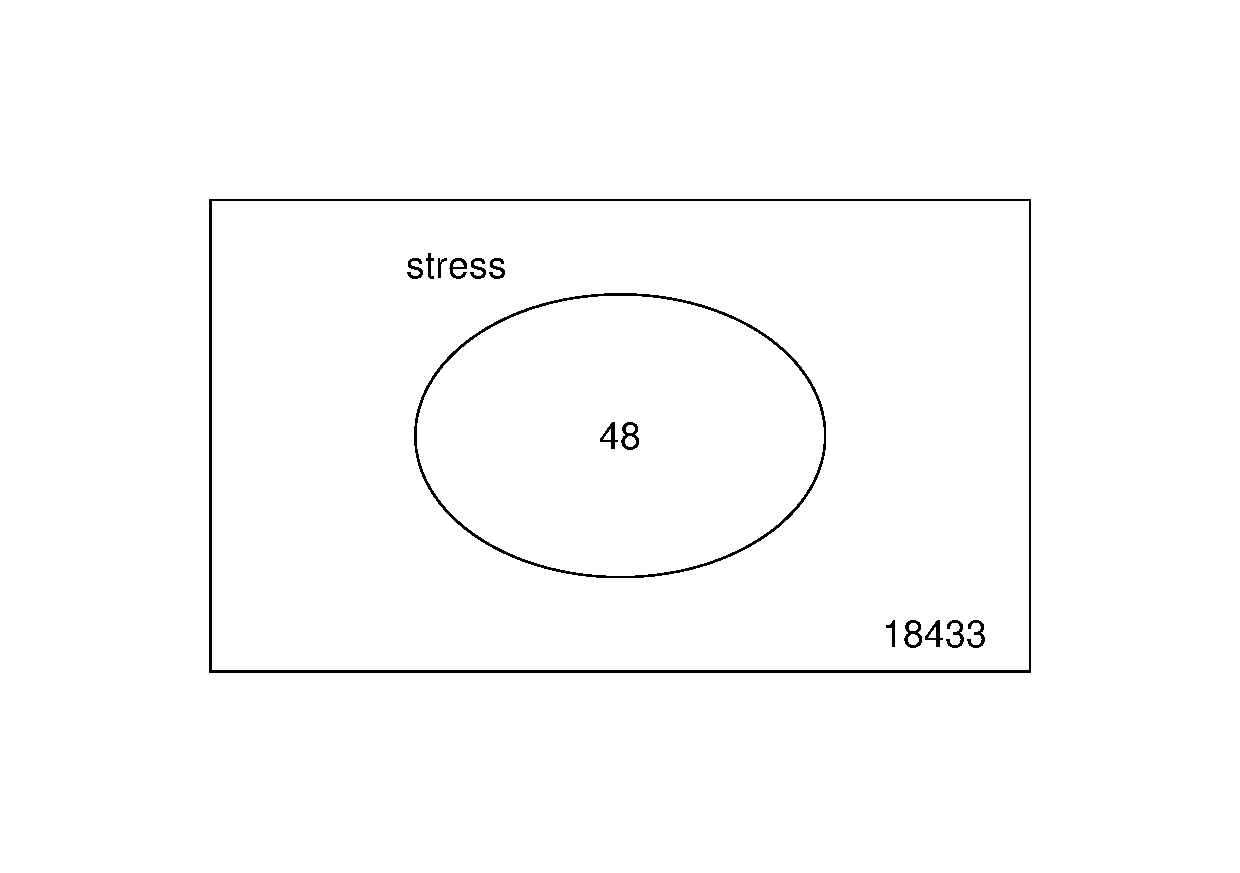
\includegraphics[width=\textwidth, height=4cm]{../../results/plots-and-tables/4.2-DEG-Venn-Diagr-Oryza_nivara}
    \end{subfigure}
    \begin{subfigure}[t]{0.44\linewidth}
        \caption{O. sativa}
        \label{fig:4.2-DEG-Venn-Diagr-Oryza_sativa}
        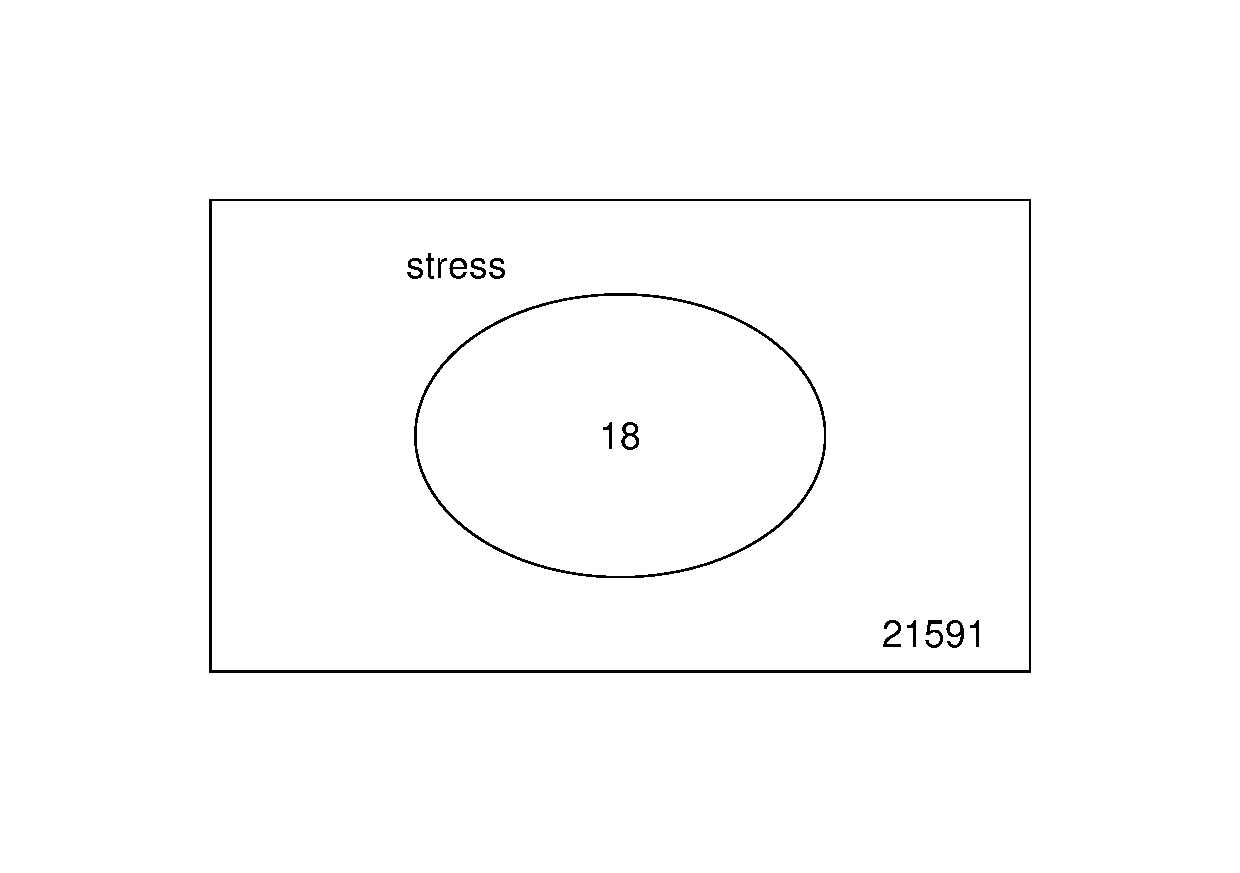
\includegraphics[width=\textwidth, height=4cm]{../../results/plots-and-tables/4.2-DEG-Venn-Diagr-Oryza_sativa}
    \end{subfigure}
\end{figure}

\begin{figure}[htbp]
    \caption{Heatmap of the DEGs - O. nivara}
    \label{fig:4.4-DEG-Heatmap-Oryza_nivara}
    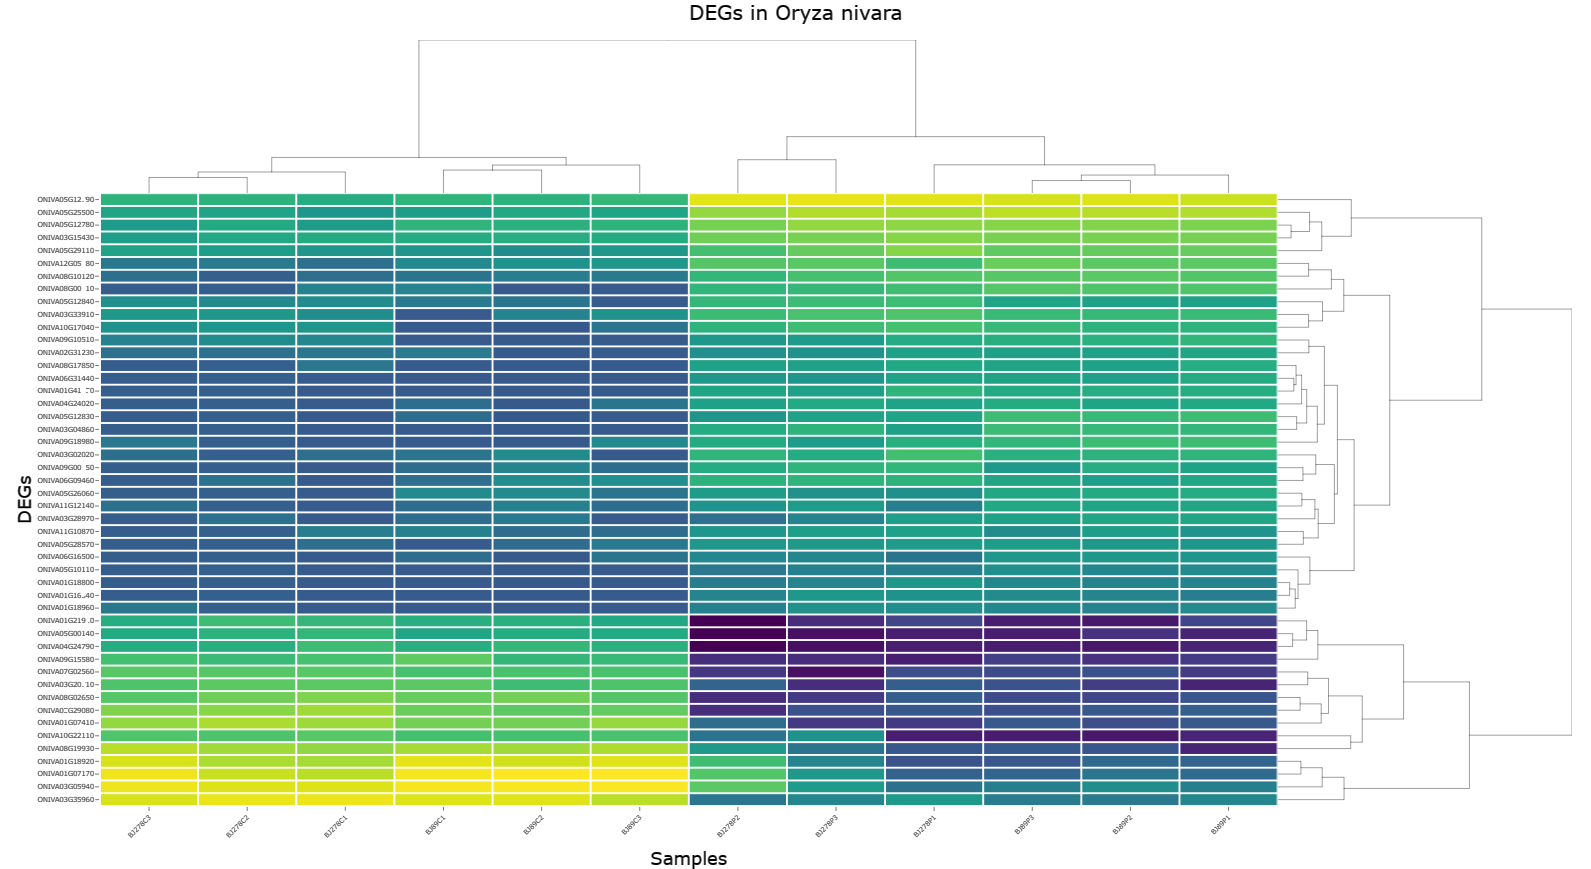
\includegraphics[width=\textwidth]{../../results/plots-and-tables/4.4-DEG-Heatmap-Oryza_nivara}
\end{figure}

\begin{figure}[htbp]
    \caption{Heatmap of the DEGs - O. sativa}
    \label{fig:4.4-DEG-Heatmap-Oryza_sativa}
    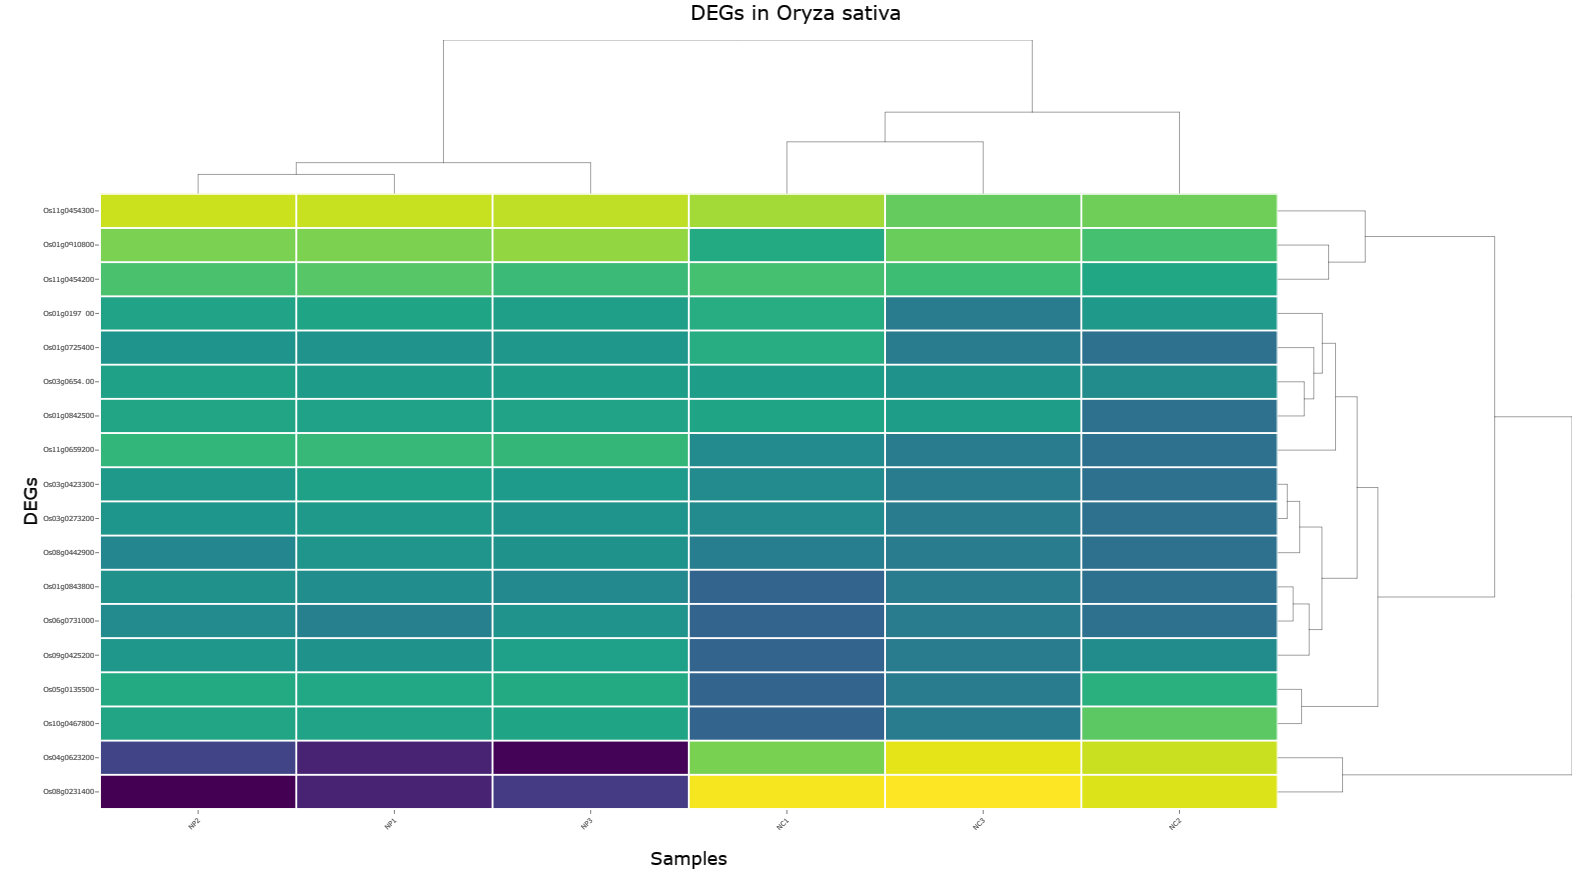
\includegraphics[width=\textwidth]{../../results/plots-and-tables/4.4-DEG-Heatmap-Oryza_sativa}
\end{figure}

\filbreak
Down- and up-regulated genes are for O. nivara:\\
{\scriptsize\texttt{ONIVA01G07170, ONIVA01G07410, ONIVA01G16640, ONIVA01G18800, ONIVA01G18920, ONIVA01G18960, ONIVA01G21950, ONIVA01G41350, ONIVA02G31230, ONIVA03G02020, ONIVA03G04860, ONIVA03G05940, ONIVA03G15430, ONIVA03G20710, ONIVA03G28970, ONIVA03G33910, ONIVA03G35960, ONIVA04G24020, ONIVA04G24790, ONIVA05G00140, ONIVA05G10110, ONIVA05G12780, ONIVA05G12790, ONIVA05G12830, ONIVA05G12840, ONIVA05G25500, ONIVA05G26060, ONIVA05G28570, ONIVA05G29080, ONIVA05G29110, ONIVA06G09460, ONIVA06G16500, ONIVA06G31440, ONIVA07G02560, ONIVA08G00310, ONIVA08G02650, ONIVA08G10120, ONIVA08G17850, ONIVA08G19930, ONIVA09G00350, ONIVA09G10510, ONIVA09G15580, ONIVA09G18980, ONIVA10G17040, ONIVA10G22110, ONIVA11G10870, ONIVA11G12140, ONIVA12G05380
}}

For O. sativa these genes are:\\
{\scriptsize\texttt{Os01g0197700, Os01g0725400, Os01g0842500, Os01g0843800, Os01g0910800, Os03g0273200, Os03g0423300, Os03g0654700, Os04g0623200, Os05g0135500, Os06g0731000, Os08g0231400, Os08g0442900, Os09g0425200, Os10g0467800, Os11g0454200, Os11g0454300, Os11g0659200
}}

A description and the location of all these genes can be found at \url{https://plants.ensembl.org}. For a deeper analysis of these genes and their potential biological significance, the available information appears to be insufficient.


\subsection{Functional enrichment analysis}

Finally, for the one-hundred top-ranked genes a statistical functional enrichment analysis\index{functional enrichment analysis} was performed to identify over- or under-represented information from gene ontology (GO)\index{gene ontology (GO)} terms. Figures \ref{fig:5.2-Gost-Plot-Oryza_nivara} and \ref{fig:5.2-Gost-Plot-Oryza_sativa} present the results as Manhattan plots.

For both O. nivara and O. sativa, the top ten GO terms belong to the major subontology "biological process (BP)"\index{gene ontology (GO)!biological process (BP)}. It appears that on the gene level the impact of drought stress may be best described and categorized in terms of biological processes as opposed to the molecular functions (MF)\index{gene ontology (GO)!molecular function (MF)} of the genes and as opposed to the cellular components (CC)\index{gene ontology (GO)!cellular component (CC)} in which the gene products are physically located.

Furthermore, for both rice species the following GO terms are significantly enriched (when just comparing the top ten GO terms): response to organic substance, response to water, response to acid chemical, response to salt, response to chemical, lignin catabolic process, phenylpropanoid catabolic process. This confirms the close relationship of the two species, and it also confirms that the GO terms are suitable to describe genetic responses to environmental factors.

\begin{figure}[htbp]
    \caption{Manhattan plot with the first 10 top-ranked GO terms highlighted - O. nivara}
    \label{fig:5.2-Gost-Plot-Oryza_nivara}
    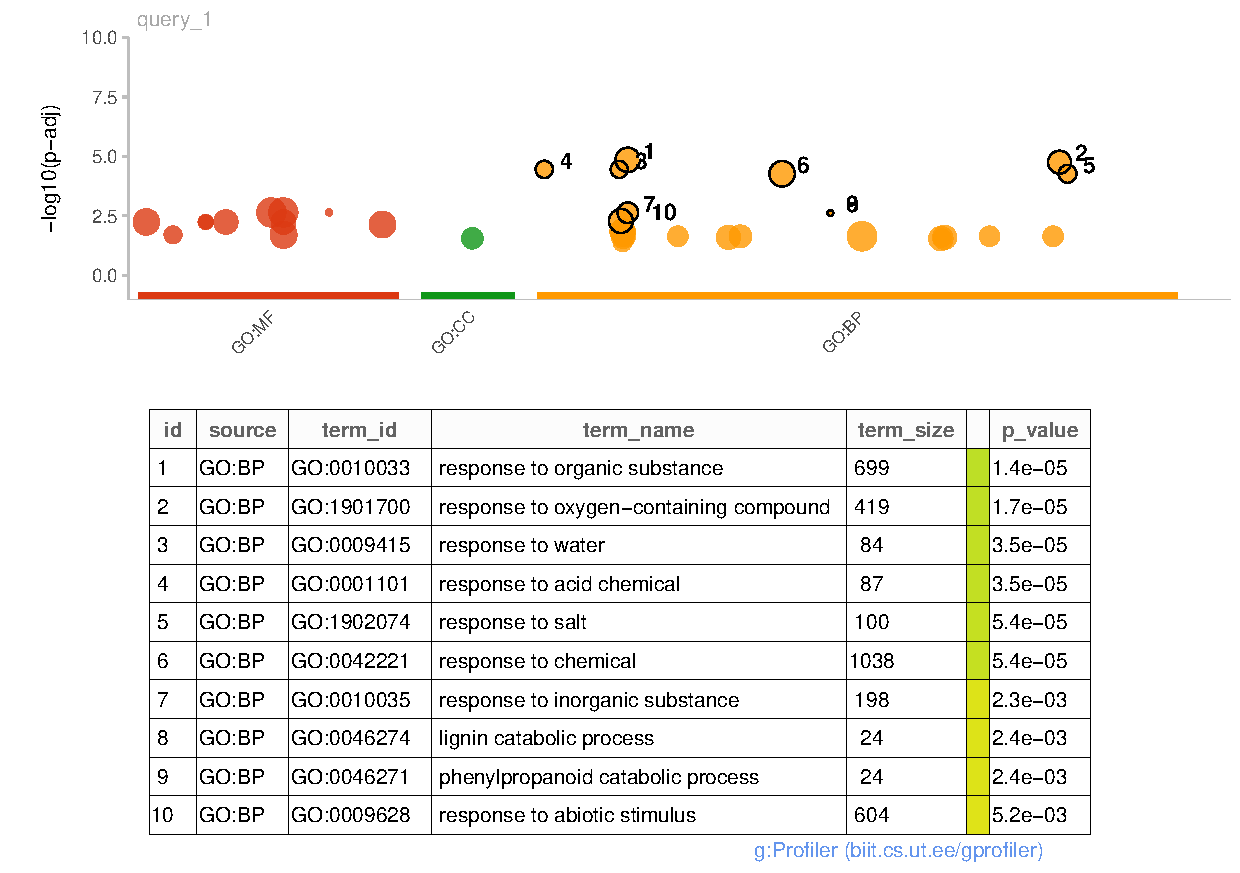
\includegraphics[width=0.9\textwidth]{../../results/plots-and-tables/5.2-Gost-Plot-Oryza_nivara}
\end{figure}

\begin{figure}[htbp]
    \caption{Manhattan plot with the first 10 top-ranked GO terms highlighted - O. sativa}
    \label{fig:5.2-Gost-Plot-Oryza_sativa}
    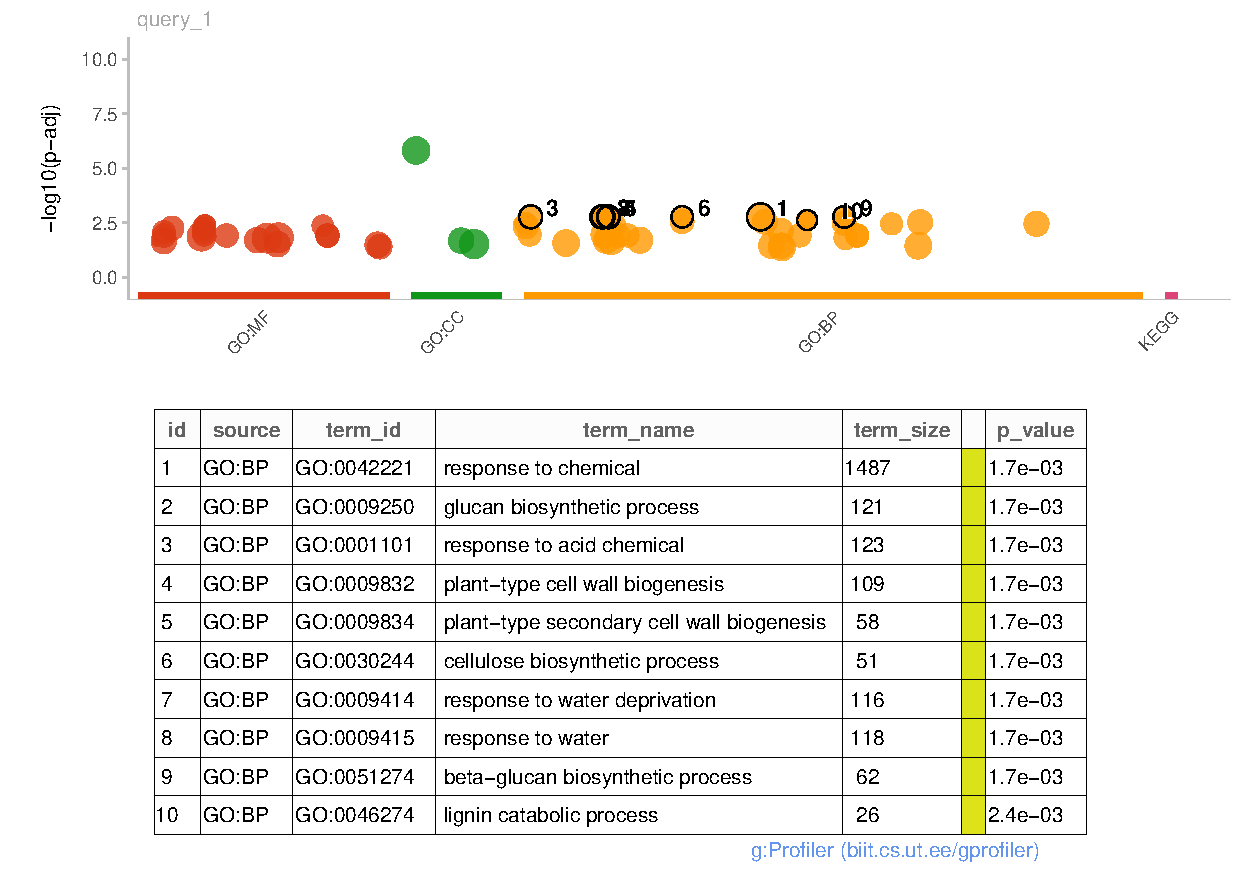
\includegraphics[width=0.9\textwidth]{../../results/plots-and-tables/5.2-Gost-Plot-Oryza_sativa}
\end{figure}

    \section{Discussion}

\subsection{Critical evaluation of the results}
Discuss the quality and reliability of the RNA-seq data and the downstream analyses.

\subsection{Biological implications}
Discuss the potential implications of the findings for plant biology and the broader scientific community.

\subsection{Limitations and future directions}
Address the limitations of the current analysis and suggest possible future directions to expand on the findings.

    \section{Conclusion}

Summarize the main findings of the assignment, reiterating the significance of the results, and provide a final statement on the overall outcome of the study.

    \newpage
    \printbibliography[heading=bibintoc]

    \newpage
    \printindex
\end{document}